% !TeX program = xelatex
\documentclass[11pt,a4paper]{article}
\usepackage[margin=25mm]{geometry}
\usepackage{amsmath,amssymb,amsthm,booktabs}
\usepackage{tikz,graphicx,longtable}
\graphicspath{{Figures/}{docs/RMFS/Papers/2026_11_SweepBasedCollisionAvoidanceFramework/Figures/}}
\usetikzlibrary{arrows.meta,positioning}
\usepackage[hidelinks]{hyperref}
\newtheorem{definition}{Definition}
\newtheorem{proposition}{Proposition}
\newtheorem{theorem}{Theorem}
\theoremstyle{remark}
\newtheorem{remark}{Remark}
\newcommand{\Sw}{\mathcal S}
\newcommand{\Rs}{\mathcal R}
\newcounter{algorithm}
\newcounter{algline}
\providecommand{\theHalgline}{\arabic{algorithm}.\arabic{algline}}
\newcommand{\algl}[3]{\refstepcounter{algline}\label{#1}\item[\arabic{algline}.]\hspace*{#2em}#3}
\newenvironment{pseudocode}[2]{%
  \par\medskip\noindent\begin{minipage}{\linewidth}\refstepcounter{algorithm}\label{#1}
  \noindent\textbf{Algorithm \thealgorithm. #2}\par\smallskip
  \hrule\smallskip\begingroup\small\setcounter{algline}{0}
  \begin{list}{}{\setlength{\leftmargin}{2em}\setlength{\labelwidth}{1.5em}\setlength{\labelsep}{.5em}\setlength{\itemsep}{3pt}}
}{\end{list}\endgroup\smallskip\hrule\end{minipage}\par\medskip}
\title{A Sweep-Based Framework for Collision Avoidance\\among Mobile Robots}
\author{Moon Ho Hwang\\\small\href{mailto:moon.hwang@gmail.com}{\texttt{moon.hwang@gmail.com}}}
\date{November 22, 2026\\\small Research working paper: theory, implementation, and examples}

\begin{document}
\maketitle
\begin{abstract}
We formulate and implement established sweep-based coordination principles for collision avoidance and finite
completion of prescribed paths by multiple mobile robots. The framework
abstracts physical time while retaining movement order: interference is
expressed through intersections of occupied-region sweeps, and compatible
movements and waits are organized into complete tuple paths. Point-sweep
duplication represents waiting, while safe sweep merging combines consecutive
movements without discarding their original control constraints. We derive
sufficient completion conditions and present construction and execution
algorithms that preserve the required interference order. Under the stated
geometric and execution assumptions, these rules provide collision-free
execution and finite completion. The formulation applies to general
occupied regions; its demonstrated realization uses two-dimensional
rectangular collision envelopes. FIFO and longest-remaining-path (LP)
policies select among admissible traffic actions without overriding the
safety and completion conditions. The theory-based control is evaluated
using Discrete Event System Specification (DEVS)
simulation~\cite{zeigler1976,zeigler2018}. A post-fix stop-only baseline
evaluates 13 fixed route sets under FIFO and LP, from three-robot inspection
cases to 50-robot mixed interior traffic with 631 directed
interference intervals totalling 2,581~m. All 26 policy conditions complete
in three repeated timed runs, with no deadlock or detected collision and matching independent
collision-stop replays. These results provide experimental validation of
the implementation and exhibit no violations of the derived safety and
completion properties. The resulting interference and completion criteria
also establish a foundation for generating optimal interference-aware
paths to new destinations. That path-generation problem will be addressed
in a subsequent study; it is not solved in this paper.
\end{abstract}

\noindent\textbf{Keywords:} Sweep Volume;  Collision 
Avoidance; Mobile Robots; Multi Robot Path Planning;
Robotic Mobile Fulfillment System (RMFS); DEVS.

\section{Introduction}

Two objects can have intersecting geometric path sweeps without colliding:
they may occupy the shared region at different times. Conversely, a move
that is collision-free while other objects wait can make later completion
impossible. Coordination therefore requires more than detecting overlap or
checking the next instantaneous configuration.

We study given ordered paths and the use of movement and waiting to execute
them. Path generation and transport-order assignment are outside the present
experiments. The initial objective is to construct complete, collision-free
executions. Completion, rather than schedule optimality, is the subject of this paper.

\paragraph{Scope of the framework and its realization.}
The title identifies mobile robots as the application studied here.
The underlying path, occupied-region, sweep and tuple definitions are not
restricted to that application: their arguments depend on the stated
geometric and execution assumptions. The demonstrated realization is
specifically two-dimensional. Robot/rack occupancy is represented by fixed
axis-aligned rectangular envelopes, and axis-aligned path segments give
rectangular sweeps. This choice makes the sweep construction and intersection
operations explicit in the implementation. Their computational cost remains
geometry-dependent in more general realizations; the experiments do not
establish an efficient sweeping algorithm for arbitrary shapes or dimensions.

The presentation follows the construction-to-execution chain:
\begin{enumerate}
\item Define paths, subpath sweeps, and complete n-object tuple paths.
\item Construct and validate a complete tuple using sufficient serial
      conditions or finite point-sweep duplication search.
\item Execute that tuple with explicit approval, feedback, release, and
      command-merging algorithms.
\item State the execution guarantees and their scope, then test the Plant
      executions and the finite classification.
\end{enumerate}
Sections~\ref{sec:construction}--\ref{sec:control-guarantees} separate the
existence of a valid witness from its construction, its execution rules,
and the guarantees justified for those rules. Simple and complex fixed-path
cases then validate two traffic-selection policies against the same safety
and completion conditions.

Residual interference groups provide a useful decomposition and monitoring
mechanism, but their monotone shrinkage is not the main research claim.
For the task-based extension, the proof sketch connects reported release
and departure guards to preservation of interference order and global
progress; numerical and physical implementation assumptions remain explicit.

\section{Relation to prior work}
\label{sec:prior-art}

\subsection{The direct predecessor: segment-sweep coordination in 1989}
O'Donnell and Lozano-P\'erez~\cite{odonnell1989} already construct
collision-free schedules for two prescribed manipulator paths using swept
volumes of ordered path segments. Their task-completion diagram records
whether pairs of segment sweeps interfere. Horizontal, vertical and diagonal
progress represent one robot advancing, the other advancing, or both
advancing. Their START/WAIT execution uses segment completion to enable
subsequent actions. Diagram cells are pairs of path segments, not cells
in a regular partition of physical space.

This is a direct predecessor of our construction, not merely research sharing
the word ``sweep.'' Printed p.~486 introduces null endpoint segments and
discusses blocking by a robot parked at its destination (Figure~3).
Printed p.~487 considers global schedule search when completing whole paths
one robot at a time is unsafe. Endpoint occupancy, waiting and alternating
partial progress therefore must not be presented as new capabilities.

\begin{table}[htbp]
\centering\small
\caption{Correspondence with the 1989 construction. Terminology alone does
not establish a different coordination principle.}
\label{tab:1989-correspondence}
\begin{tabular}{p{.29\linewidth}p{.62\linewidth}}
\toprule
Present terminology & Established counterpart~\cite{odonnell1989}\\\midrule
Partial-path sweep & Swept volume of an ordered path segment.\\[3pt]
Point sweep and final occupancy & Null endpoint segment and persistent endpoint blocking.\\[3pt]
Compatible sweep pair & Compatible segment-pair cell in the task-completion diagram.\\[3pt]
Point-wait duplication & Hold one progress coordinate while the other advances.\\[3pt]
Alternating partial progress & Alternate horizontal and vertical schedule progress.\\[3pt]
Untimed execution order & Segment-completion-driven START/WAIT commands.\\
\bottomrule
\end{tabular}
\end{table}

\paragraph{An explicit finite-model correspondence.}
Fix two paths with $m_i,m_j$ edges, admissible vertex stops, footprints
and a conservative sweep-intersection predicate. Define
\begin{equation}
\begin{split}
 Q_{ij}&=\{0,\ldots,m_i\}\times\{0,\ldots,m_j\},\\
 (k,l)&\longrightarrow(k+d_i,l+d_j)
 \quad\Longleftrightarrow\quad
 \Sw_i[k,k+d_i]\cap\Sw_j[l,l+d_j]=\varnothing.
\end{split}
\label{eq:prior-progress}
\end{equation}
Here $(d_i,d_j)\in\{(1,0),(0,1),(1,1)\}$, successors remain inside
$Q_{ij}$, and $\Sw_i[k,k]$ is the waiting footprint at vertex $k$.
Only in this comparison, sweep arguments count edges rather than using
the normalized parameter introduced below. Initial footprints must be
disjoint; final footprints persist.

Our exhaustive point-duplication model and this adapted classical
segment-progress graph have the same completion reachability for the fixed
finite input. In one direction, erase point-token consumption that does not
advance a robot: each remaining stage is a permitted progress step. In the
other direction, insert the original point tokens at safe vertices before
and after each progress step while the other robot waits. Their footprints
are subsets of the corresponding safe step sweeps. Both transformations
preserve path order and safety. This is a correspondence of the finite
models, not a claim about unrestricted synchronized continuous motion or
about the original authors' implementation.

Point duplication therefore does not establish a new two-robot feasibility
principle. Our sixteen endpoint classes are a restricted characterization,
not a replacement for the broader segment-conflict scheduling problem
already addressed in 1989. The identical four-bit table was not located in
the inspected sources; that observation does not establish novelty.

\subsection{Subsequent coordination and feedback execution}
Leroy et al.~\cite{leroy1999} address multiple mobile robots through geometric
coordination diagrams and interaction decomposition; their allowed controls
include backward progress, unlike our forward-only finite model.
Gr\'egoire et al.~\cite{gregoire2015}, Section~3.2, Theorem~3, prove
feasibility of acyclic priorities by topologically ordering robots and
letting them finish serially. This is the same constructive proof pattern
as our acyclic sufficient construction, subject to different geometric and
endpoint assumptions.

RMTRACK~\cite{cap2016} preserves a known coordinated passage order under
delaying disturbances. ADG~\cite{hoenig2019} uses action-completion reports
and combines consecutive forward commands while retaining feedback.
Segment Graph~\cite{coskun2021} partitions trajectories at interference
boundaries and examines deadlock after passage-order changes; its
non-conflicting-trajectory condition excludes other robots' starts/goals.
SADG~\cite{berndt2024} uses MILP to reorder permissible dependencies and
establishes recursive feasibility under stated assumptions. These overlap
our order-preserving control, reported release and sweep-merging ideas.
Constructing an initial valid plan and executing it remain separate tasks.

\subsection{Time-based passage-order repair: what the controller can learn}
\label{sec:time-repair-review}
Coskun and O'Kane~\cite{coskun2019}, Section~V, address the observed case:
a robot waits because another has priority, although it might clear the
shared region before that robot arrives. A flip check is made the first
time a particular obstacle blocks progress, at most once per obstacle for
that robot. TestFlipFast compares expected clearance and arrival times
using the coordination obstacle's bounding box. TestFlipAggressive models
joint progress and compares the sum of the two robots' expected clearance
times under the existing and reversed labels. This is local expected-time
evaluation, not full-fleet makespan optimization. Disturbance estimates
are learned through Gaussian-process regression. Crucially, a successful
test changes the obstacle's priority label; RMTRACK still governs movement.
The expected-time comparison is a performance criterion, not a deterministic
guarantee that the region will be vacant for that entire predicted interval.

\begin{figure}[htbp]
\centering
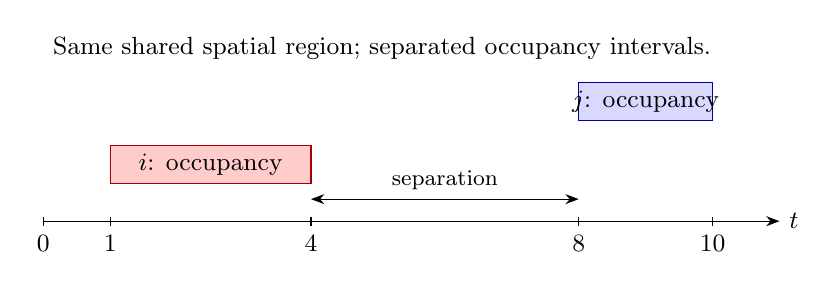
\begin{tikzpicture}[x=.85cm,y=.8cm,>=Stealth,every node/.style={font=\small}]
\draw[->] (0,0)--(11,0) node[right] {$t$};
\foreach \x in {0,1,4,8,10} {\draw (\x,.07)--(\x,-.07) node[below] {\x};}
\filldraw[fill=red!20,draw=red!65!black] (1,.6) rectangle (4,1.2);
\node at (2.5,.9) {$i$: occupancy};
\filldraw[fill=blue!15,draw=blue!65!black] (8,1.6) rectangle (10,2.2);
\node at (9,1.9) {$j$: occupancy};
\draw[<->] (4,.35)--node[above,font=\footnotesize]{separation}(8,.35);
\node[anchor=west] at (0,2.75) {Same shared spatial region; separated occupancy intervals.};
\end{tikzpicture}
\caption{Illustrative times, not experimental data. Geometric sweep overlap
alone need not require waiting. Predicted separation must be distinguished
from enforceable passage order and bounded timing uncertainty.}
\label{fig:timed-separation}
\end{figure}

The later Segment Graph paper~\cite{coskun2021}, Definitions~2--4 and its
algorithm description, supplies the missing multi-robot check. Vertices
represent path portions split at interference boundaries. Edges preserve
own-path order and impose finish-before-start relations between robots.
A proposed flip rewires the affected precedence; a cycle check rejects
changes that introduce circular waiting. Its no-cycle/deadlock implication
requires trajectories that avoid every other robot's initial and final
position. Figure~4 explicitly shows endpoint blocking without a graph cycle.
Consequently we cannot transfer that guarantee to arbitrary new order legs
or occupied workstation endpoints merely by running a cycle detector.
The model also uses discrete steps and disc robots; its controller is not
a direct implementation for our continuous acceleration profiles.

\paragraph{A proposed adaptation, not an implemented guarantee.}
For a particular shared region $C$, distinguish estimated relative times
$\widehat{\tau}^{\rm clear}_{i,C}$ and
$\widehat{\tau}^{\rm enter}_{j,C}$ from certified bounds. The fast
performance test is
\begin{equation}
 \widehat{\tau}^{\rm clear}_{i,C}
 < \widehat{\tau}^{\rm enter}_{j,C}.
 \label{eq:estimated-gap}
\end{equation}
A stronger, sufficient timing certificate would instead require
\begin{equation}
 \overline{\tau}^{\rm clear}_{i,C}+\eta
 <\min_{j\ne i}\underline{\tau}^{\rm enter}_{j,C},
 \label{eq:bounded-gap}
\end{equation}
over all robots able to enter $C$, where the upper bound covers the admitted
robot's latest full-footprint clearance, the lower bound covers each other's
earliest entry, and $\eta$ is an additional nonnegative time margin.
This is our proposed engineering criterion, not a theorem attributed to
the two papers. Arbitrarily long delays invalidate a finite clearance upper
bound. Alternatively, enforce the new order by holding other robots outside
$C$ until actual clearance, while validating their ability to stop there.

The useful design sequence is therefore: identify the local interference
portions; estimate whether a change is worthwhile; validate its precedence,
endpoint and stopping conditions; record the changed reservation atomically;
then execute using actual clearance reports. Already-issued movement commands
cannot be silently revoked. Downstream blocking must also be included in
the clearance estimate or excluded by reservation. Our current TrafficManager
does not yet implement this time-aware order repair; this paragraph specifies
what must be checked before adding it. It neither authorizes an unsafe early
departure nor claims a general completion guarantee for dynamically added legs.

\subsection{The decision instant: before braking rather than after stopping}
\label{sec:prebraking-review}
The proposed follow-up has a more precise timing question than whether
acceleration is modeled: can a robot decide to continue through the next
interference region before it begins braking for the preceding stopping point?
Under the deterministic virtual-twin assumption, this decision would branch
the current moving state, rather than a state already at rest.

\paragraph{A direct precedent for the braking-boundary event.}
Quesel et al.~\cite{quesel2016}, Section~5.3, Example~3a, explicitly model
an event-triggered stop-sign controller using the boundary
\begin{equation}
 p+\frac{v^2}{2B}=S,
 \label{eq:braking-boundary}
\end{equation}
where $p$ is position along the lane, $v$ is speed, $B>0$ is the braking
deceleration magnitude and $S$ is the stopping position. The controller
must execute no later than this boundary, although it may execute earlier.
This is direct evidence that invoking control at the final feasible braking
point is established. It is a stop-sign safety example, not a simulation-based
multi-robot crossing authorization algorithm. Section~5.5 also distinguishes
ideal event detection from sampled sensing. Our virtual-twin assumption
permits the ideal event to be scheduled analytically; it does not make the
boundary principle new.
This final feasible braking boundary need not coincide with the earlier
start of a chosen comfort-oriented deceleration profile; the selected braking
model and stopping point must be stated when comparing decision instants.

\paragraph{Simulation-based admission before arrival.}
Dresner and Stone~\cite{dresner2008}, Sections~3.3--3.4 and Appendix~C,
let an approaching driver request an arrival time and speed. The intersection
manager simulates traversal against existing space-time tile reservations.
Acceptance reserves that passage; rejection causes the driver to decelerate
and request again. This already combines pre-entry simulation with the
possibility of avoiding a stop, including acceleration alternatives.
The reviewed procedure does not identify one mandatory invocation exactly
at Equation~\eqref{eq:braking-boundary}. Its candidate traversal simulation
against reservations is also different from cloning an entire DEVS fleet.
Neither that difference nor replacing tiles with sweeps establishes novelty.

\paragraph{A direct precedent for brake-line-dependent stop/go behavior.}
Kalose et al.~\cite{kalose2024}, Sections~5.1--5.2 and Figure~5,
compute braking lines from speed and chosen deceleration levels. Their
tactical state machine selects passage or phased braking from the vehicle's
position relative to those lines and the traffic-light state. A green signal
allows passage without intersection-induced slowing. This directly relates
the decision to the approaching vehicle's braking geometry. It is a
signalized-intersection controller, not residual-sweep conflict evaluation
or a full-state snapshot lookahead.

\begin{table}[htbp]
\centering\small
\caption{Which part of the proposed pre-braking lookahead is actually
supported by the inspected sources. No row asserts identity of full algorithms.}
\label{tab:prebraking-review}
\begin{tabular}{p{.24\linewidth}p{.33\linewidth}p{.34\linewidth}}
\toprule
Source & Directly relevant result & Distinction from our proposal\\\midrule
Quesel et al.~\cite{quesel2016} & Invoke control at or before the final braking boundary.
& Stop-sign safety, not crossing simulation.\\[4pt]
Dresner--Stone~\cite{dresner2008} & Simulate and reserve passage before entry; decelerate if denied.
& Candidate traversal against reservations, rather than a cloned fleet; no mandatory braking-boundary trigger identified.\\[4pt]
Kalose et al.~\cite{kalose2024} & Stop/go decisions tied to speed and braking lines.
& Traffic-light input, not fleet snapshot evaluation.\\[4pt]
Proposed DEVS study & Branch the moving snapshot at a scheduled pre-braking event; test clearance of the next region.
& Not yet implemented or validated; novelty unestablished.\\
\bottomrule
\end{tabular}
\end{table}

\paragraph{The specific experiment still to perform.}
For the simple constant-braking model, define the forward distance to the
selected safe stopping position as $d_i(t)$. The decision event solves
$d_i(t_b)=v_i(t_b)^2/(2b_i)$ with $v_i(t_b)>0$ and $b_i>0$; an earlier
configured trigger may use additional distance. For more general motion
profiles the appropriate stopping-distance function replaces this expression.
At $t_b$, snapshot both position and velocity plus controller state. Simulate
the continue alternative until the robot's complete envelope clears the next
interference region. If it cannot clear safely, follow the braking branch
to the stopping point. Match the accepted branch's commands and reservations
in the parent execution. This is a proposed local passability test, not a
proof of full-route completion. A turn that physically requires zero speed
cannot be eliminated by obtaining passage permission.

Compare this policy against deciding only after stopping, measuring stop
count, delay, completion time, lookahead calls and wall-clock cost. The
inspected literature establishes the individual ideas of braking-boundary
control and simulation-based pre-entry permission. An identical combination
with this particular DEVS snapshot and local termination condition has not
been established by this focused reading; absence from these selected papers
is not evidence of historical priority.

\paragraph{The precise difference to investigate.}
The proposed method is not distinguished by ``using acceleration'' or
``simulating before permission'': those elements have the precedents above.
Its intended combination has three specified features:
\begin{enumerate}
\item \textbf{Decision trigger.} Schedule the decision at the beginning of the
selected stop-to-stop profile's braking portion, while the robot is moving,
rather than requiring it to reach the stop point first. Quesel's final feasible
braking boundary and Kalose's braking lines are relevant timing precedents;
the mere use of a position/speed event is not a novelty claim.
\item \textbf{Evaluated state.} Restore a fleet snapshot including positions,
velocities, ongoing motions, pending DEVS events, reservations and controller
state. Execute the continue alternative with a specified continuation policy.
This differs from Dresner--Stone's traversal test against an existing
reservation table. Whether cloning the additional state changes decisions or
only increases evaluation cost must be measured, not assumed.
\item \textbf{Local termination.} Evaluate through full-envelope clearance of
the next interference region, not through completion of every robot's path.
This local target limits the test's claim to that passage; it does not remove
the need to preserve downstream feasibility separately.
\end{enumerate}
These are proposed design differences from the inspected formulations,
not validated advantages or a claim that no other publication combines them.
Under the virtual-twin assumption, accepted parent execution must retain the
branch's commands, reservations and decision rules; otherwise a successful
branch does not justify the actual continuation.

An informative experiment must separate the effect of \emph{when to decide}
from \emph{how to evaluate}. Use identical paths, footprints and motion limits
to compare stop-then-decide with pre-braking decisions, and compare a
reservation-based passage evaluator with the full-state twin evaluator at
the same decision instants. A matched reference implementation must be
identified as an adaptation unless the original published implementation is
reproduced. Report disagreements in permission decisions, avoided stops,
waiting time, completion time and per-decision runtime. If the two evaluators
always agree, the evidence supports a different implementation or computational
trade-off, not an additional coordination capability. This investigation
remains future work; no pre-braking twin advantage is established here.

\subsection{SCALE and the meaning of inclusion}
The reviewed SCALE manuscript~\cite{scale2026} integrates roadmap planning
and local repair, heterogeneous geometric conflict checks, an action
precedence graph (HAPG), action capsules, and bounded-horizon MILP passage-order
adjustment. Its footprint sweep includes translation and rotation. Finite
bit occupancy does not by itself imply a regular physical workspace grid.

Our alternating-progress witness is representable in HAPG: using the same
square envelope and feasible action ranks gives four inter-robot edges,
whose transitive reduction has the same two dependencies as the corresponding
ADG construction. The apparent robot-level cycle disappears when different
actions retain their own dependencies. This analytical compilation is not
an execution of SCALE's planner or MILP. It shows that our example does not
demonstrate a missing capability in these graph representations.

SCALE has broader system functionality than our reported fixed-path study:
route generation/repair and passage-order optimization are included.
Its displayed MILP minimizes summed predicted horizon-exit times, not
full-operation makespan. A different objective or a full-Plant simulator
does not by itself establish a new coordination principle.

\begin{figure}[htbp]
\centering
\resizebox{\linewidth}{!}{%
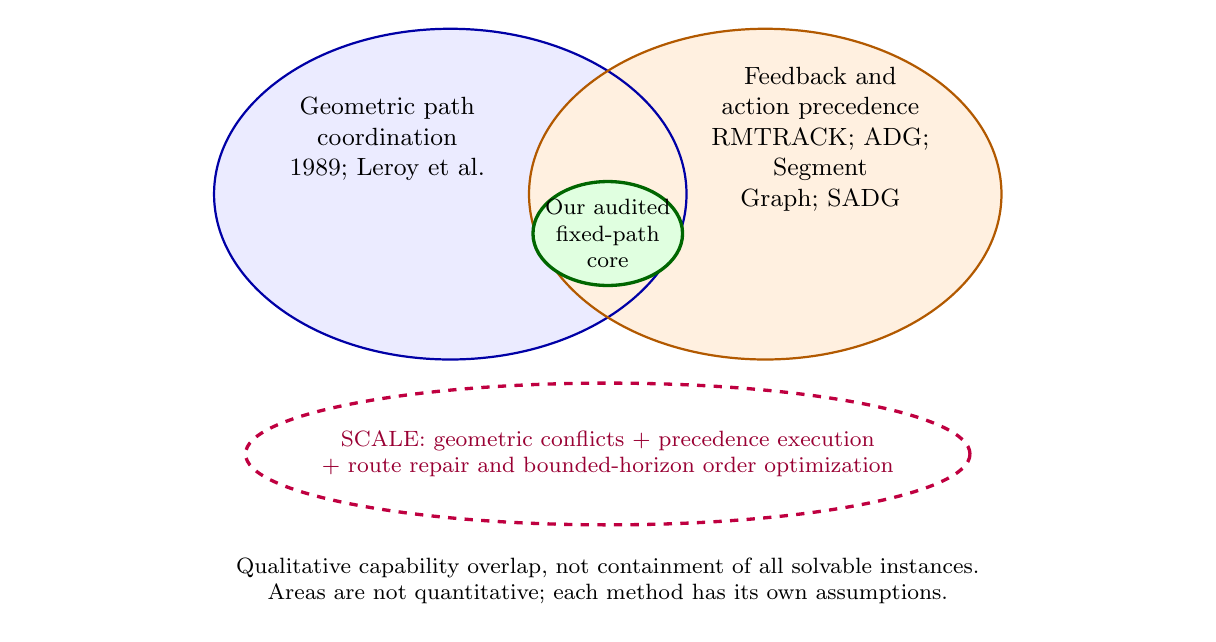
\begin{tikzpicture}[every node/.style={font=\small,align=center}]
\fill[blue!8] (3,2) ellipse (3 and 2.1);
\fill[orange!12] (7,2) ellipse (3 and 2.1);
\draw[thick,blue!65!black] (3,2) ellipse (3 and 2.1);
\draw[thick,orange!70!black] (7,2) ellipse (3 and 2.1);
\node[text width=30mm] at (2.2,2.7) {Geometric path\\coordination\\1989; Leroy et al.};
\node[text width=32mm] at (7.7,2.7) {Feedback and\\action precedence\\RMTRACK; ADG;\\Segment Graph; SADG};
\draw[very thick,green!40!black,fill=green!12] (5,1.5) ellipse (.95 and .66);
\node[text width=18mm,font=\footnotesize] at (5,1.5) {Our audited\\fixed-path\\core};
\draw[very thick,dashed,purple] (5,-1.3) ellipse (4.6 and .9);
\node[text width=80mm,font=\footnotesize,purple!80!black] at (5,-1.3) {SCALE: geometric conflicts + precedence execution\\+ route repair and bounded-horizon order optimization};
\node[anchor=north,text width=145mm,font=\footnotesize] at (5,-2.5)
{Qualitative capability overlap, not containment of all solvable instances.\\
Areas are not quantitative; each method has its own assumptions.};
\end{tikzpicture}}
\caption{Venn-style map of conceptual overlap. The green region locates the
established principles used by our implementation, not a newly established
theoretical region. The diagram is not a formal algorithm-inclusion theorem.}
\label{fig:prior-art-overlap}
\end{figure}

\paragraph{Supported inclusion and unproved inclusion.}
Equation~\eqref{eq:prior-progress} gives a reachability correspondence for
our fixed two-robot finite abstraction. Its core principles are established
segment-sweep coordination. Our alternating witness is also representable
in existing action graphs. However, a universal solved-instance inclusion
$\mathcal F_{\rm ours}\subseteq\mathcal F_{\rm SCALE}$ has not been proved:
footprints, stops, initial/final occupancy, allowed motions, search coverage,
horizons and timeouts must first be aligned. More system features do not
prove that every instance solved by one program is solved by another.

The confirmed differences are the explicit endpoint table, point-token
bookkeeping, rectangular RMFS realization and timed DEVS Plant. No independent
theoretical advantage, superior speed, or non-overlapping theoretical
contribution is currently established. Implementation and experiment
records remain useful without implying that the underlying coordination
problem was previously unsolved.

\subsection{Geometry and implementation evidence}

\paragraph{Cell-based conflicts and physical occupancy.}
A representative warehouse formulation by H\"onig et al.~\cite{hoenig2019},
Sections~III--IV, uses a four-connected grid and discrete vertex/edge
conflicts for planning, then an action dependency graph for continuous-time
execution. Its cell size, robot diameter and restricted actions connect
that abstraction to physical safety. The limitation is therefore not that
cell methods are inherently unsafe: their conflict rules depend on these
geometric assumptions. On a different aisle graph, two distinct edges can
have overlapping robot or rack sweeps; different cell identifiers alone
cannot establish physical separation. Conversely, a coarse reserved cell
can exclude physically disjoint movements. Extending such a formulation
requires suitable footprints, inflated regions or additional conflicts.

MiR600 illustrates the practical motivation for separating motion geometry
from logical traffic resources. Its manufacturer describes map-based global
planning and local obstacle avoidance~\cite{mir600guide}, rather than a
requirement to move between four neighbouring warehouse cells. This does
not assert that its internal maps contain no discretization. Our claim is
that the coordination framework need not impose a regular workspace grid.

\paragraph{Geometric coordination and its computational cost.}
Sweeps and fixed-path coordination already have substantial foundations
\cite{odonnell1989,leroy1999,gregoire2015,cap2016}. Leroy et
al.~\cite{leroy1999}, Sections~4--5, explicitly avoid a regular workspace
grid and report up to 150 robots. Their reported efficiency depends on
interaction-group decomposition: a large connected group raises the
dimension of the coordination search, and they identify approximately ten
robots as the practical group dimension in their implementation.
Separately, \AA blad et al.~\cite{ablad2021} identify distance-query cost in
swept-path verification and reduce it through adaptive clearance sampling;
their results favour this over explicit octree sweep intersection.
These works identify two distinct scaling costs: geometric queries and
combinatorial coordination. They do not establish that sweep methods
cannot be applied to RMFS or that scalability alone explains industrial
adoption.

\paragraph{Position of this work.}
We connect sweep-based tuple construction, order-preserving execution and
report-driven residual release in one reproducible implementation. General
occupied-region definitions are realized here with inexpensive rectangular
sweeps of axis-aligned 2D segments. Experiments include 50 mobile robots
and a nonuniform warehouse aisle graph with twenty loaded robots.
The same timed Plant and controller also drive an interactive 3D animation,
so physical motion and reported residual release can be inspected during
execution. The engineering result is this theory-to-execution realization and its measured
performance, not the first non-grid coordination method or the largest
fleet: large-scale cell-based warehouse planning has already been reported
for 1,000 agents~\cite{li2021}. Section~\ref{sec:contributions} relates our
specific evidence to these different modeling and computational choices.

\section{Geometric model and sweep operations}

\begin{definition}[Paths and occupied regions]
Object $i\in\{1,\ldots,n\}$ has a fixed continuous path
\begin{equation}
 P_i:[0,1]\longrightarrow\mathcal Q_i,\qquad
 s_i=P_i(0),\quad e_i=P_i(1).
 \label{eq:path}
\end{equation}
The parameter $u$ is ordered progress, not physical time.
$B_i(u)\subseteq\mathbb R^d$ is the nonempty region occupied at $P_i(u)$.
For $0\le a\le b\le1$, define
\begin{equation}
 P_i^{[a,b]}=P_i|_{[a,b]},\qquad
 \Sw_i[a,b]=\bigcup_{u\in[a,b]}B_i(u).
 \label{eq:sweep}
\end{equation}
\end{definition}

Objects advance monotonically or wait. Geometry, assigned paths, object
dimensions, and any safety inflation are fixed during an execution.
Contact counts as interference. A point sweep is
$\Sw_i[a,a]=B_i(a)$, not an empty set.
Numerical time is introduced for physical execution and performance, while
the geometric reasoning retains order without requiring precise timing.

\paragraph{RMFS geometry.}
The current backend uses a fixed axis-aligned rectangle. A rectangle moving
along an axis-aligned segment produces a rectangular sweep; a polyline
produces a union of rectangles. The rack does not rotate when its supporting
robot turns. We use the configured rack-sized envelope even for an empty
robot, a conservative modeling choice in these tests.

The rectangular approximation is an approximation of physical occupancy.
For the adopted fixed rectangle and axis-aligned translation, the union of
segment rectangles is its geometric sweep, rather than a time-sampling
approximation. In the experiments, $B_i(u)$ denotes this chosen collision
envelope. Its interpretation as a conservative physical bound requires
\begin{equation}
 B_i^{\mathrm{phys}}(u)\subseteq B_i(u)\quad\text{for every }u
 \quad\Longrightarrow\quad
 \Sw_i^{\mathrm{phys}}[a,b]\subseteq\Sw_i[a,b].
 \label{eq:physical-envelope}
\end{equation}
Thus disjoint envelope sweeps imply disjoint physical sweeps when the
containment condition holds throughout the motion. Rotation or other
configuration changes must be included in that condition. The general
framework requires suitable occupied-region and sweep-intersection operations;
the rectangular backend is the particular realization validated here.

\begin{figure}[htbp]
\centering
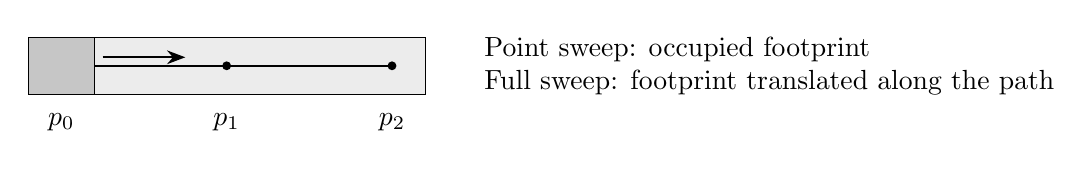
\begin{tikzpicture}[x=1.05cm,y=.9cm,>=Stealth]
\filldraw[fill=gray!15] (-.4,-.4) rectangle (4.4,.4);
\draw[thick] (0,0)--(2,0)--(4,0);
\foreach \x in {0,2,4} {\fill (\x,0) circle (1.6pt);}
\draw[thick,->] (.5,.12)--(1.5,.12);
\draw[fill=gray!45] (-.4,-.4) rectangle (.4,.4);
\node at (0,-.8) {$p_0$};\node at (2,-.8) {$p_1$};\node at (4,-.8) {$p_2$};
\node[align=left,right] at (5,0) {Point sweep: occupied footprint\\
Full sweep: footprint translated along the path};
\end{tikzpicture}
\caption{A fixed rectangular footprint and its straight-path sweep. The
intermediate point remains part of the original path even if passed without stopping.}
\label{fig:sweep}
\end{figure}

\begin{definition}[Paired and tuple paths]
A finite tuple path is a sequence of stages
\begin{equation}
 \mathcal T=(\mathcal P^{(1)},\ldots,\mathcal P^{(m)}),\qquad
 \mathcal P^{(k)}=(P_1^{[a_1^{(k)},b_1^{(k)}]},\ldots,
                    P_n^{[a_n^{(k)},b_n^{(k)}]}),
 \label{eq:tuple}
\end{equation}
where $a_i^{(1)}=0$, $b_i^{(m)}=1$,
$b_i^{(k)}=a_i^{(k+1)}$, and $a_i^{(k)}\le b_i^{(k)}$.
The case $n=2$ is a paired path. A point component denotes waiting while
other components of that stage execute.
\end{definition}

\paragraph{Point-sweep duplication.}
Copying and inserting a point component represents additional waiting. It
does not duplicate a moving path portion or change the original path.
The untimed representation does not assign a numerical duration to that wait.

\paragraph{Sweep merging and splitting.}
Merging joins adjacent subpaths of the same object in their original order.
It removes an intermediate stopping boundary without deleting the original
vertex or replacing a bend by a shortcut. Splitting restores an existing
intermediate vertex as a stopping boundary; it does not insert a new geometric
point. The implementation includes a split function, but the reported control
experiments do not use a separate splitting operation to modify the control plan.

\section{Constructing complete tuple paths}
\label{sec:construction}
The construction problem is to produce a finite tuple covering every
original path whose stages satisfy
\begin{equation}
 \Sw_i[a_i^{(k)},b_i^{(k)}]\cap
 \Sw_j[a_j^{(k)},b_j^{(k)}]=\varnothing\qquad(i<j),
 \label{eq:stage-safe}
\end{equation}
This is a geometric, order-based requirement: no duration is assigned to a
point wait. We first give sufficient serial constructions, then a finite
partial-progress search, and finally a safe merging transformation. Their
execution guarantee is established in Section~\ref{sec:control-guarantees}.

\subsection{Two-object endpoint test}
Define four indicators for the full paths:
\begin{equation}
 \sigma_{i|j}=\mathbf1\{B_i(0)\cap\Sw_j[0,1]\ne\varnothing\},\qquad
 \varepsilon_{i|j}=\mathbf1\{B_i(1)\cap\Sw_j[0,1]\ne\varnothing\}.
 \label{eq:flags}
\end{equation}
The test
\begin{equation}
 F_{ij}=(\neg\sigma_{j|i}\land\neg\varepsilon_{i|j})
       \lor(\neg\sigma_{i|j}\land\neg\varepsilon_{j|i})
 \label{eq:pair-test}
\end{equation}
is sufficient for a complete serial execution of two objects.
\begin{proof}
For the first term, object $j$ can wait at its start while $i$ completes,
and $i$ can then wait at its goal while $j$ completes. Both moving-versus-waiting
intersections are empty by the indicators. The second term reverses the roles.
\end{proof}

For arbitrary paths, failure of~\eqref{eq:pair-test} does not prove
infeasibility: alternating partial progress can succeed. The 16-type finite
classification reported below concerns a restricted unit-pair domain,
not a necessary-and-sufficient test for arbitrary footprints and paths.

\subsection{Acyclic requirements for multiple objects}
Create a directed requirement graph with
\begin{equation}
 i\longrightarrow j\quad\Longleftrightarrow\quad
 \sigma_{j|i}=1\ \text{or}\ \varepsilon_{i|j}=1.
 \label{eq:precedence}
\end{equation}
The arrow means that this serial construction requires $j$ before $i$.
In this graph, $F_{ij}=0$ is equivalent to the reciprocal edges
$i\to j$ and $j\to i$. Hence acyclicity already implies $F_{ij}=1$ for
every pair. The converse fails for three or more objects: pairwise success
excludes two-object cycles, but not longer cycles.


\begin{theorem}[Acyclic sufficient construction]
\label{thm:dag}
If this graph is acyclic, an ordering that executes every required predecessor
first gives a complete, collision-free serial execution, assuming each path
can be executed in finite time.
\end{theorem}
\begin{proof}
When $i$ moves, every other object $j$ is either waiting at its initial
configuration or has finished. If $j$ is scheduled later, an intersection
between $B_j(0)$ and $i$'s full sweep would imply $i\to j$, contrary to the
ordering. If $j$ is scheduled earlier, an intersection between $B_j(1)$ and
$i$'s full sweep would imply $j\to i$, again contrary to the ordering.
Thus each move avoids every stationary object. Initial or final overlap of
two objects would itself create reciprocal requirements, so it is excluded
by acyclicity. Finite sequential completion follows.
\end{proof}

This condition is not necessary. A static requirement cycle can sometimes
be resolved by partial progress or concurrent movement. A static requirement
graph is neither the undirected interference graph nor the current wait-for graph.


\subsection{Constructing and validating a tuple path}
The preceding tests provide inexpensive sufficient constructions, not a
necessary admission rule for every input. In particular, a static cycle
does not prevent a search from constructing a tuple by alternating partial
progress. Algorithm~\ref{alg:construction} summarizes this finite search.
The implementation is the \texttt{solve} method of
\texttt{WaitDuplicationSolver}; its \texttt{validate} method checks the
returned witness before a controller is created.

Let $w_i=(p_{i,0},e_{i,01},p_{i,1},\ldots,p_{i,m_i})$ be the original
point/edge constituent word and $c_i$ the number of consumed constituents.
A search state $c=(c_1,\ldots,c_n)$ records progress, not time. Selecting an
object consumes its next constituent; not selecting it inserts a point wait
at its current vertex. Selected constituents may themselves be points.

\begin{pseudocode}{alg:construction}{Construct a complete tuple by point-sweep duplication}
\algl{ln:search-input}{0}{\textbf{Input:} fixed paths, footprints, geometry policy and words $w_i$.}
\algl{ln:search-precheck}{0}{Reject overlapping initial/final footprints or reversed object order on a common straight line.}
\algl{ln:search-init}{0}{Enqueue $c=(0,\ldots,0)$; mark it visited with an empty predecessor.}
\algl{ln:search-pop}{0}{\textbf{While} the FIFO queue is nonempty: remove its first state $c$.}
\algl{ln:search-goal}{1}{\textbf{If} $c_i=|w_i|$ for all $i$: reconstruct, independently validate, and return the tuple.}
\algl{ln:search-subsets}{1}{\textbf{For each} nonempty subset $M$ of objects with unconsumed items:}
\algl{ln:search-row}{2}{Form a row using $w_i[c_i]$ for $i\in M$ and a current point wait otherwise.}
\algl{ln:search-safe}{2}{\textbf{If} all row sweep pairs are disjoint: form $c'_i=c_i+\mathbf1\{i\in M\}$.}
\algl{ln:search-enqueue}{3}{\textbf{If} $c'$ is unvisited: store its predecessor and row, mark it visited, and enqueue it.}
\algl{ln:search-failure}{0}{Return failure when the queue is exhausted; omit all-wait self-loops.}
\end{pseudocode}

The independent validation checks the initial and final counts, consumption
without skips, exact original constituents, point-only inserted waits, and
all-pair sweep disjointness in every row. Thus the witness supplies both
coverage and~\eqref{eq:stage-safe}. Breadth-first search is complete for this
finite constituent model; it does not minimize physical makespan or claim
completeness over arbitrary continuous partial-path stopping positions.

\paragraph{Algorithm 1: correctness, completeness, and termination.}
Every accepted transition consumes only next original constituents and
inserts only point waits (lines~\ref{ln:search-row}--\ref{ln:search-safe}).
The pairwise test on line~\ref{ln:search-safe} establishes the stage condition.
The goal test and independent validation on line~\ref{ln:search-goal}
establish full coverage, so any returned tuple is correct.
For completeness within the finite model, every productive valid stage
selects some nonempty subset enumerated on line~\ref{ln:search-subsets}.
An all-wait row can be removed without changing reachability. Induction on
the number of productive stages shows that every reachable state is visited
or already has a recorded predecessor. Thus exhaustion on
line~\ref{ln:search-failure} means no witness exists in this model.
The preliminary rejections on line~\ref{ln:search-precheck} are sound because
all objects must coexist at their initial/final footprints and forward-only
objects on one straight line cannot exchange order without contact.

There are at most $N_s=\prod_i(|w_i|+1)$ states; line~\ref{ln:search-enqueue}
enqueues each once. Each state has at most $2^n-1$ subset choices, each using
finitely many geometric tests. Hence the search terminates. With cached
constituent sweeps and pair-test cost bounded by $G$, a coarse time bound is
$O(N_s2^n n^2G)$ and predecessor/queue memory is $O(N_s n)$, apart from
geometry caches. This is a finite exhaustive method, not a claim of
scalability or makespan optimality. Without the prechecks, breadth-first
search returns a witness with minimum productive stage count in this state
graph; that count is not physical duration.

For the larger acyclic examples, \texttt{dag\_witness} instead repeatedly
selects objects whose required predecessors have completed, forms a batch
with mutually disjoint full sweeps, and consumes their constituent words
while the others wait. It returns a tuple checked by the same validator.
The admission tests and this constructive route are sufficient; cyclic
candidates rejected by that generator are not declared generally infeasible.

\subsection{Safe merging of n-object tuple stages}
For two adjacent stages, the merged component sweep is
\begin{equation}
 U_i=\Sw_i[a_i^{(k)},b_i^{(k)}]\cup
     \Sw_i[a_i^{(k+1)},b_i^{(k+1)}].
 \label{eq:merged-union}
\end{equation}
The conservative merge condition is
\begin{equation}
 U_i\cap U_j=\varnothing\qquad\text{for every }i<j.
 \label{eq:merge-safe}
\end{equation}
If both original stages are individually safe, the extra checks are
\begin{equation}
 \Sw_i[a_i^{(k)},b_i^{(k)}]\cap
 \Sw_j[a_j^{(k+1)},b_j^{(k+1)}]=\varnothing\qquad(i\ne j).
 \label{eq:merge-cross}
\end{equation}
By Proposition~\ref{prop:ordered}, such a merged stage preserves ordered
execution safety and completion if its movements finish in finite time.
This is a sufficient geometric rule, not a complete search for every possible
safe temporal overlap or an optimal merge policy.

\section{Executing a validated tuple path}
\label{sec:execution}
The input to the traffic controller is the validated tuple from
Section~\ref{sec:construction}, not just a collection of independently safe
next moves. The following rules explain how that witness becomes Plant
commands and how progress feedback permits further execution.


\begin{figure}[htbp]
\centering
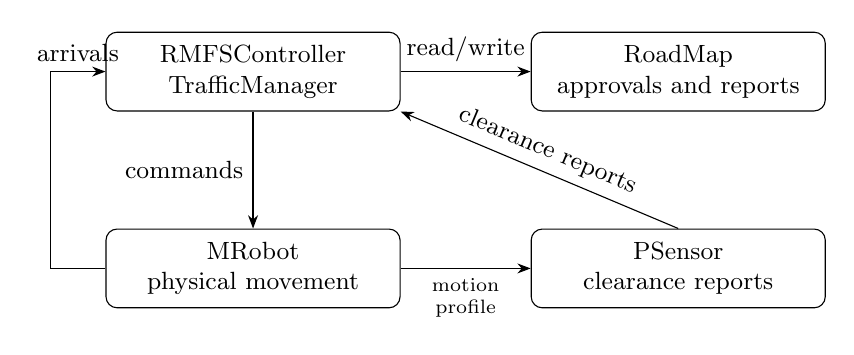
\begin{tikzpicture}[>=Stealth,every node/.style={font=\small},
 block/.style={draw,rounded corners,align=center,text width=3.5cm,minimum height=1cm}]
\node[block] (manager) at (0,1.4) {RMFSController\\TrafficManager};
\node[block] (road) at (5.4,1.4) {RoadMap\\approvals and reports};
\node[block] (robot) at (0,-1.1) {MRobot\\physical movement};
\node[block] (sensor) at (5.4,-1.1) {PSensor\\clearance reports};
\draw[->] (manager)--node[above]{read/write}(road);
\draw[->] (manager)--node[left]{commands}(robot);
\draw[->] (robot)--node[below,align=center,font=\scriptsize]{motion\\profile}(sensor);
\draw[->] (sensor.north)--node[sloped,above]{clearance reports}(manager.south east);
\draw[->] (robot.west)--++(-.7,0)|-node[pos=.75,above]{arrivals}(manager.west);
\end{tikzpicture}
\caption{One physical robot and one sensor per object, with a single controller.
TrafficManager and RoadMap are ordinary controller-owned objects, not extra
Plant DEVS models. Sensor reports are received by the controller, which
updates RoadMap and reconsiders departures.}
\label{fig:architecture}
\end{figure}

\subsection{Roles and state}
The coupled RMFS model contains one RMFSController and an MRobot/PSensor
pair per object. MRobot and PSensor are DEVS atomic models. TrafficManager
generates commands; RMFSController emits them from a buffer. RoadMap is a
shared blackboard distinguishing approved movement from physically reported
progress. Approval does not teleport an object.

MRobot approximates MiR600 motion using acceleration, constant-speed travel
when the distance permits, and deceleration, rather than constant-speed
motion alone. The manufacturer's published maximum speed is
$2\,\mathrm{m/s}$~\cite{mir600}; the numerical approximation and its assumptions
are specified below.

PSensor is introduced to avoid the excessive periodic position communication
of a discrete-time sensing simulation. It schedules only meaningful
footprint-clearance reports analytically from the commanded motion profile,
without a fixed sensing-time step or control-point entering reports.
MRobot reports final command arrival and rotation
events. Traffic decisions occur on these events rather than a periodic
control-time loop. Numerical sampling is used for display and optional
collision validation, not as the departure-control clock.

The motion-profile equations, parameter values, and phase transitions are detailed in Appendix~\ref{app:plant-models}.

\subsection{Departure approval and release}
Every non-point component of the validated tuple becomes a movement task
$q=(k,i,P_i^{[a,b]})$, with stage $k$, owner $i$, and sweep $C(q)$.
Original tasks remain unchanged when commands are merged. An unissued task
retains its full sweep; an issued task retains its unpassed sweep.
At conservatively reported progress $\hat u_i$, RoadMap retains
\begin{equation}
 \Rs_i(\hat u_i)=\Sw_i[\hat u_i,1],\qquad \Rs_i(1)=B_i(1).
 \label{eq:residual}
\end{equation}
Thus final arrival retains occupancy. Reports must be monotone and must
not advance beyond actual progress.

\begin{pseudocode}{alg:permission}{Permit one movement task}
\algl{ln:guard-input}{0}{\textbf{Input:} next task $q$ of an idle robot and current RoadMap.}
\algl{ln:guard-prior}{0}{Reject if an earlier own task is unfinished.}
\algl{ln:guard-interference}{0}{Reject if $C(q)$ intersects an earlier unfinished other-robot task's retained sweep.}
\algl{ln:guard-occupancy}{0}{Reject if $C(q)$ intersects another robot's active residual command sweep or idle footprint.}
\algl{ln:guard-yes}{0}{Otherwise permit $q$.}
\end{pseudocode}
Only unpassed interference constrains departure: clearing a shared region
can enable another robot before the first command ends. Required occupancy
order, rather than a global stage barrier, is preserved.

\subsection{Event-driven dispatch and merging}
\begin{pseudocode}{alg:dispatch}{Dispatch and update from Plant reports}
\algl{ln:dispatch-input}{0}{\textbf{On initialization, clearance, or arrival:} update RoadMap and completed original tasks; retain final footprints.}
\algl{ln:dispatch-loop}{0}{Visit idle robots' next requests in the selected FIFO or LP order.}
\algl{ln:dispatch-guard}{1}{Skip a blocked request using Algorithm~\ref{alg:permission}; otherwise begin a command prefix.}
\algl{ln:dispatch-extend}{1}{If merging is enabled, extend within a validated merge block while every added task passes the same approval checks.}
\algl{ln:dispatch-approve}{1}{Reserve the prefix in RoadMap and mark its tasks issued before buffering the command.}
\algl{ln:dispatch-issued}{0}{RMFSController emits buffered commands; reconsider waiting requests on subsequent Plant reports.}
\algl{ln:dispatch-done}{0}{Finish when every original movement task is completed.}
\end{pseudocode}
Merge blocks satisfy~\eqref{eq:merge-safe}. A blocked extension does not
hold back its permitted prefix. Merging changes command boundaries and
motion profiles, not approval units or release conditions. Rotation reports
update monitoring; clearance and arrival reports drive dispatch without
periodic polling. Collision-stop validation halts on a detected contact.

\subsection{FIFO and LP within permitted orders}
\label{sec:two-policies}
To allow alternative admissible orders, retain a finite nonempty family
$\mathcal V$ of validated complete tuples over the same original tasks.
For candidate $q$, define its supporting certificates by
\begin{equation}
 \mathcal V(q)=\{\Pi\in\mathcal V:
 C(q)\text{ avoids all unpassed earlier other-robot reservations in }\Pi\}.
 \label{eq:certificate-support}
\end{equation}
Approval requires nonempty support, own-path order, and the physical
occupancy check in Algorithm~\ref{alg:permission}; the earlier-task check
is evaluated within each supporting tuple. On approval retain only
$\mathcal V(q)$. Every task of a merged prefix must share a common nonempty
support set. A single reference tuple is the case $|\mathcal V|=1$.

Let $a_i$ be a request's first waiting time and let
\begin{equation}
 \ell_i(q_i)=\operatorname{len}(P_i^{[q_i,1]})
 \label{eq:policy-length}
\end{equation}
be remaining polyline length in metres at waiting position $q_i$.
\begin{itemize}
\item \textbf{FIFO:} send a sole eligible arrival immediately; when several
eligible robots wait for a released region, select the earliest $a_i$.
\item \textbf{LP:} select the largest remaining $\ell_i$, with FIFO ties.
A first arrival may wait for a longer-path robot only if that robot has an
already-approved finite approach to a safe waiting position. Compare lengths
at the waiting positions, excluding the approach distance; equal lengths
send the first arrival. Among eligible approaching partners select the
largest waiting-position length.
\end{itemize}
Waiting positions are original vertices before interference. The held
footprint must not obstruct the committed approach. Each ordered pair of
waiting positions may cause at most one intentional hold; arrival ends
that hold and the same policy selects among all eligible waiters.
Neither policy overrides occupancy or certificate support, and neither
is claimed to minimize completion time.

\section{Order preservation and finite completion}
\label{sec:control-guarantees}
\label{sec:algorithm-proof}
Assume a validated finite tuple (or finite nonempty family of tuples),
matching occupied envelopes, forward traversal, conservative progress
reports, finite execution and report delivery for every issued command,
and processing of enabled dispatch/output events. Commands have finitely
many reports; no external halt occurs.

\begin{proposition}[Safe execution and finite completion]
\label{prop:ordered}
\label{prop:controller}
\label{prop:policy-completion}
Under these assumptions, Algorithms~\ref{alg:permission} and~\ref{alg:dispatch},
including the certificate-preserving FIFO and LP rules, complete the
prescribed paths without collision in finite time.
\end{proposition}
\begin{proof}[Proof sketch]
\textbf{Safety and order.} Induct over approvals. The own-task check
(line~\ref{ln:guard-prior}) preserves path order. Retained predecessor sweeps
preserve required interference order; the physical check
(line~\ref{ln:guard-occupancy}) excludes active and idle occupancy.
Reservation precedes command emission (line~\ref{ln:dispatch-approve}),
so subsequent approvals see the new commitment. Conservative release only
removes passed regions and retains endpoints. Merged prefixes apply the
same checks to every task (line~\ref{ln:dispatch-extend}). For alternative
orders, the common nonempty support set preserves at least one complete
tuple compatible with all approvals.

\textbf{Progress.} After active commands and intentional holds drain,
choose any retained tuple and its first unfinished movement task $q$.
Earlier tasks in that tuple are finished. A robot still at its corresponding
stage position cannot obstruct $q$, by tuple validation. A robot advanced
beyond that stage cannot obstruct it either: its approved sweep, including
its endpoint, had to avoid the then-unpassed $C(q)$ in the retained tuple.
Thus $q$ passes the guards and dispatch cannot remain permanently idle.
An LP hold ends in finite time because it waits only for an already-committed
safe approach; each waiting-position pair causes at most one hold.

\textbf{Termination.} Every command issues at least one new original task.
With $K$ tasks there are at most $K$ commands, finitely many reports and
intentional holds, each completed in finite time. The finite scans in
Algorithms~\ref{alg:permission} and~\ref{alg:dispatch} terminate, and the
progress argument excludes an unfinished permanently idle state.
All prescribed paths therefore finish in finite time.
\end{proof}
The guarantee concerns the stated geometric and execution assumptions.
The experiments below test the implementation; numerical collision checks
are not a continuous-time proof or a verification of real hardware.

\section{Illustrative examples}

\subsection{Two objects requiring alternating partial progress}
In grid-index coordinates, let
\begin{align}
 P_1 &: (0,1)\to(2,1)\to(2,3)\to(3,3),\nonumber\\
 P_2 &: (2,3)\to(0,3)\to(0,1)\to(0,0).
 \label{eq:alternating}
\end{align}
Intermediate adjacent grid vertices are retained in the implemented paths.
Each grid unit is 2m. Neither full path can finish while the other object
stays at its initial configuration: each path passes the other's start.
Nevertheless, the following ordered construction succeeds:
\begin{enumerate}
\item R1 moves to $(2,1)$ while R2 waits at $(2,3)$.
\item R2 completes its path while R1 waits at $(2,1)$.
\item R1 completes its remaining path while R2 waits at $(0,0)$.
\end{enumerate}
The three moving-versus-waiting sweep pairs are disjoint for the configured
footprint. This is a geometric witness, not a claim that every automatic
controller must choose this exact schedule.

\begin{figure}[htbp]
\centering
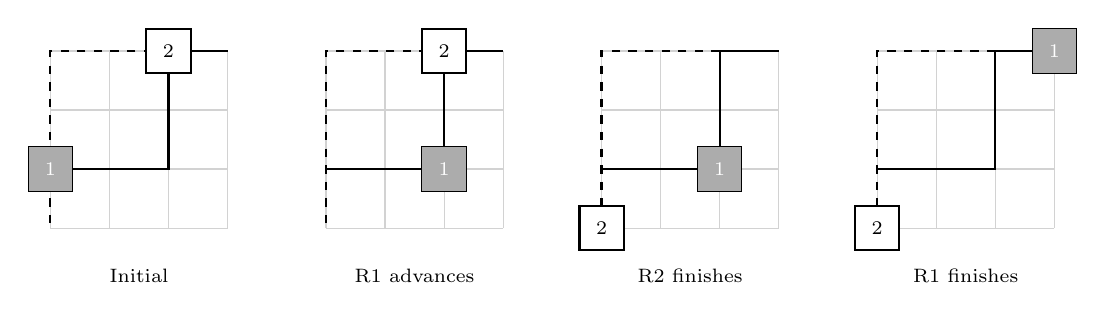
\begin{tikzpicture}[>=Stealth,every node/.style={font=\scriptsize}]
\foreach \panel/\shift/\ax/\ay/\bx/\by/\caption in
 {0/0/0/1/2/3/{Initial},1/3.5/2/1/2/3/{R1 advances},
  2/7/2/1/0/0/{R2 finishes},3/10.5/3/3/0/0/{R1 finishes}} {
 \begin{scope}[xshift=\shift cm,x=.75cm,y=.75cm]
 \draw[step=1,gray!35] (0,0) grid (3,3);
 \draw[thick] (0,1)--(2,1)--(2,3)--(3,3);
 \draw[thick,dashed] (2,3)--(0,3)--(0,1)--(0,0);
 \draw[fill=gray!65] (\ax-.375,\ay-.375) rectangle (\ax+.375,\ay+.375);
 \draw[fill=white,thick] (\bx-.375,\by-.375) rectangle (\bx+.375,\by+.375);
 \node[text=white] at (\ax,\ay) {1};\node at (\bx,\by) {2};
 \node at (1.5,-.8) {\caption};
 \end{scope}
}
\end{tikzpicture}
\caption{Alternating-progress witness. Gray and white squares mark the
objects' 1.5m square collision envelopes. Solid and dashed lines distinguish
the paths in monochrome.}
\label{fig:alternating}
\end{figure}

\subsection{Three objects and transitive interference}
Add a third path
\begin{equation}
 P_3:(3,0)\to(3,1)\to(2,1)\to(2,0)
 \label{eq:third}
\end{equation}
to the previous pair. The initial full-sweep graph has edges $\{1,2\}$ and
$\{1,3\}$, but no edge $\{2,3\}$. All three objects belong to one component
even though not every pair interferes. Thus pairwise noninterference of R2
and R3 does not justify separating them from their shared interaction with R1.

Both examples were rerun with merging and clearance-driven departure, empty
motion parameters, collision checking, and collision stopping enabled.
Table~\ref{tab:small} reports the actual automatic executions rather than
assigning durations to the explanatory witness above.

\begin{table}[htbp]
\centering
\caption{Historical illustrative executions with 0.01-second collision checks, recorded before the latest motion/sensor fixes. These are not the post-fix baseline measurements.}
\label{tab:small}
\begin{tabular}{lrrrr}
\toprule
Example & Objects & FIFO commands & FIFO (s) & LP (s)\\
\midrule
Alternating progress & 2 & 4 & 23.499 & 23.499\\
Three-object interference & 3 & 7 & 28.086 & 28.086\\
\bottomrule
\end{tabular}
\end{table}

\section{Finite endpoint-classification experiment}

On a 4$\times$4 point grid with 2m spacing and 1.5m square footprints, all
nontrivial simple paths of at most five edges produce 1,616 paths.
The experiment checks 1,799,096 ordered pairs after excluding initial
overlaps and disconnected common centerline intersections. The accepted
domain allows an empty intersection or one connected common centerline
subpath. This domain restriction is essential.

Table~\ref{tab:classification} uses bits
$(\sigma_{i|j},\varepsilon_{i|j},\sigma_{j|i},\varepsilon_{j|i})$.
An independent finite reachability check agreed with the endpoint formula
for every accepted pair. A further 320 representative cases were
cross-checked against the production solver. These are finite experimental
results, not a necessary-and-sufficient theorem for arbitrary paths.

\begin{table}[htbp]
\centering
\caption{Endpoint-type counts in the restricted finite experiment.}
\label{tab:classification}
\begin{tabular}{lrr@{\qquad}lrr}
\toprule
Bits & $F_{ij}$ & Count & Bits & $F_{ij}$ & Count\\
\midrule
0000 & 1 & 654,464 & 1000 & 1 & 176,144\\
0001 & 1 & 176,144 & 1001 & 1 & 113,488\\
0010 & 1 & 176,144 & 1010 & 0 & 42,280\\
0011 & 0 & 12,656 & 1011 & 0 & 5,064\\
0100 & 1 & 176,144 & 1100 & 0 & 12,656\\
0101 & 0 & 113,488 & 1101 & 0 & 10,128\\
0110 & 1 & 113,488 & 1110 & 0 & 5,064\\
0111 & 0 & 10,128 & 1111 & 0 & 1,616\\
\bottomrule
\end{tabular}
\end{table}

The experiment's discrete reachability oracle and its production cross-check
are separate implementations. Their agreement tests implementation and
classification consistency within the stated model, not the completeness of
all possible continuous-time coordination schemes.

\section{Validation from simple crossings to dense traffic}
\label{sec:validation}
\subsection{Case construction and measured complexity}
The historical example collection contains 81 admitted path cases: 60 seeded generated cases and
21 fixed examples. Each has at least one independently validated complete
tuple; certificate families retain the same fixed paths and movement
tasks. The reported generated families use seeds beginning at 20261120.
Those earlier data comprise ten cases each at 4, 8, 12 and 16 objects on a fixed
$12\times12$ grid, ten six-object waypoint-detour cases on a $16\times16$
grid, and ten eight-object self-avoiding random-path cases on a
$20\times20$ grid. Existing routes remain unchanged as the 12-grid cases
grow from 4 to 8, 12 and 16 objects. Admission uses geometric feasibility
and certificate validation, not the eventual policy outcome.

All grid counts denote vertices, not cells. Spacing is 2~m and the fixed
collision envelope is $1.5\times1.5$~m, including unloaded motion. Empty
motion uses acceleration/deceleration $0.41\,\mathrm{m/s^2}$, maximum speed
$2\,\mathrm{m/s}$ and angular speed $45$ degrees/s. Runs use one physical
MRobot/PSensor pair per object and one RMFSController. The same geometry,
motion parameters, completion certificates and stopping boundaries are
used for FIFO and LP.

Let $\mathcal I_{i|j}$ be the connected progress intervals of $P_i$ whose
object sweep intersects the full sweep of $P_j$. We report
\begin{equation}
 K_I=\sum_{i\ne j}|\mathcal I_{i|j}|,\qquad
 L_I=\sum_{i\ne j}\sum_{I\in\mathcal I_{i|j}}\operatorname{len}(P_i|_I).
 \label{eq:validation-complexity}
\end{equation}
These are directed pairwise counts and path-length sums in metres.
A region interfering with several opponents is counted per opponent;
$L_I$ is neither area nor a merged spatial-union length. The two
directions of a pair need not have equal interval counts. These measured
quantities, rather than object count alone, describe the examples' geometric
interference. They do not define a general computational-hardness measure.

\subsection{What the example types mean}
Figure~\ref{fig:case-gallery} shows actual initial Panda3D viewer captures
with white backgrounds, the same Iso view and translucent prescribed
sweeps. The green MRobot bodies are rendered as Frogeye (Frogy); formal
claims concern their fixed collision envelopes, not their decorative eyes.
\begin{itemize}
\item \textbf{Single crossing:} two routes cross in one shared region.
\item \textbf{Alternating progress:} one whole-route serial order is
insufficient; one object advances partially, the other passes, and the first continues.
\item \textbf{Three-object chain:} one route interferes with each of two
others, creating a coupled three-object problem.
\item \textbf{Multiple interference groups:} several objects share corridor
portions; the five-object fixture contains two interference groups.
\item \textbf{Perimeter convoy:} objects follow overlapping portions of a
cyclic road, while each individual path remains simple and finite.
\item \textbf{Interior mixed traffic:} objects traverse the interior in
mixed directions with turns. The dense family uses a constructed complete
simultaneous-matching witness; it is not obtained by exhaustive state search.
\end{itemize}
\begin{figure}[p]
\centering
\begin{minipage}{.48\linewidth}\centering
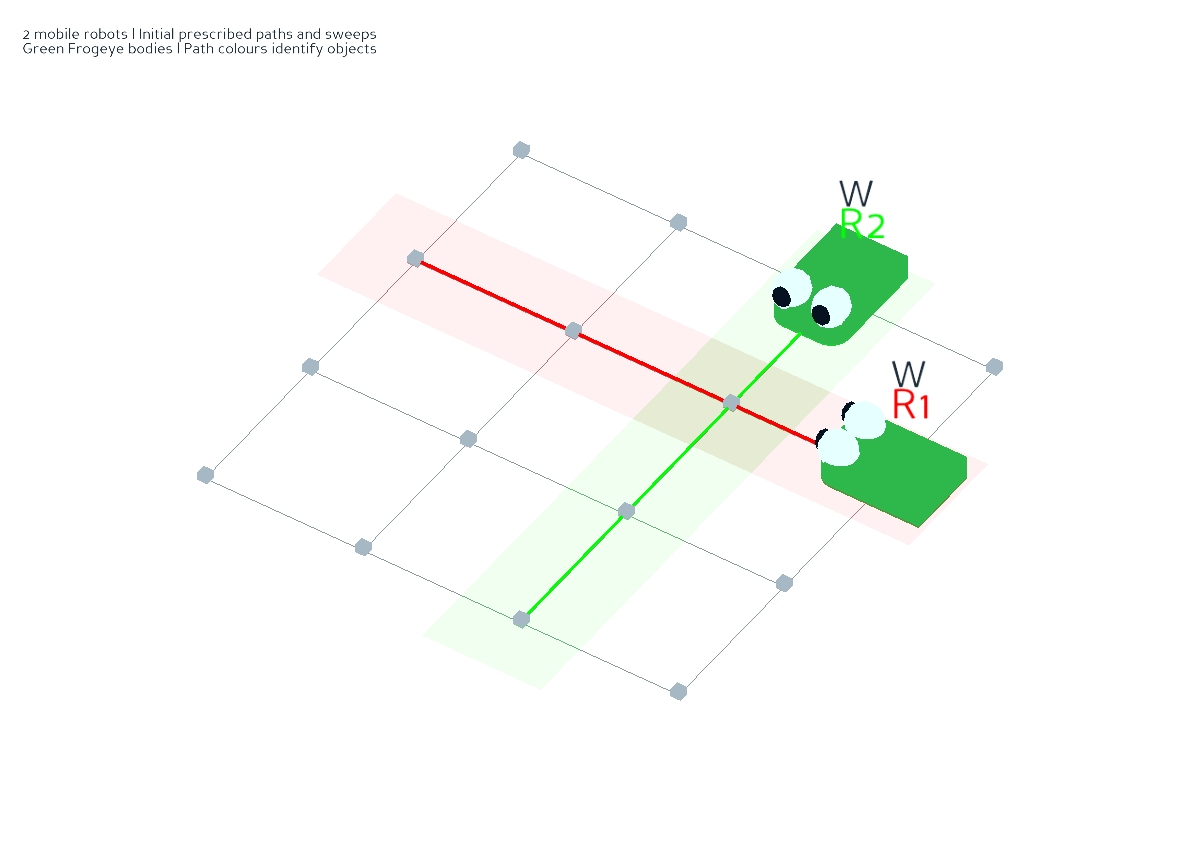
\includegraphics[width=\linewidth]{paper_02_01_RobotPath_Crossing_NoControl.png}
\par\small (a) Single crossing: 2 objects.\par\scriptsize $4\times4$, $K_I=2$, $L_I=6$~m.
\end{minipage}\hfill
\begin{minipage}{.48\linewidth}\centering
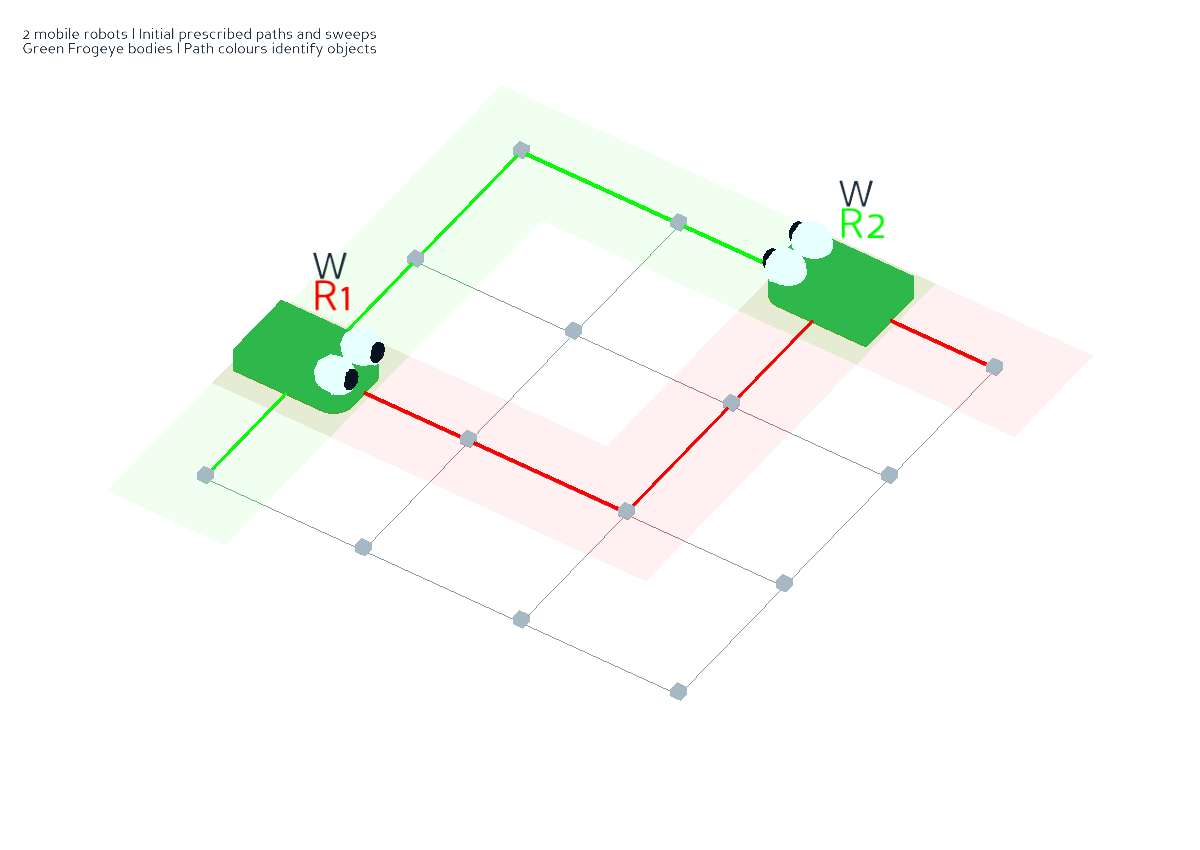
\includegraphics[width=\linewidth]{paper_02_10_RobotPath_AlternatingProgress.png}
\par\small (b) Alternating partial progress: 2 objects.\par\scriptsize $4\times4$, $K_I=4$, $L_I=9$~m.
\end{minipage}\par\medskip
\begin{minipage}{.48\linewidth}\centering
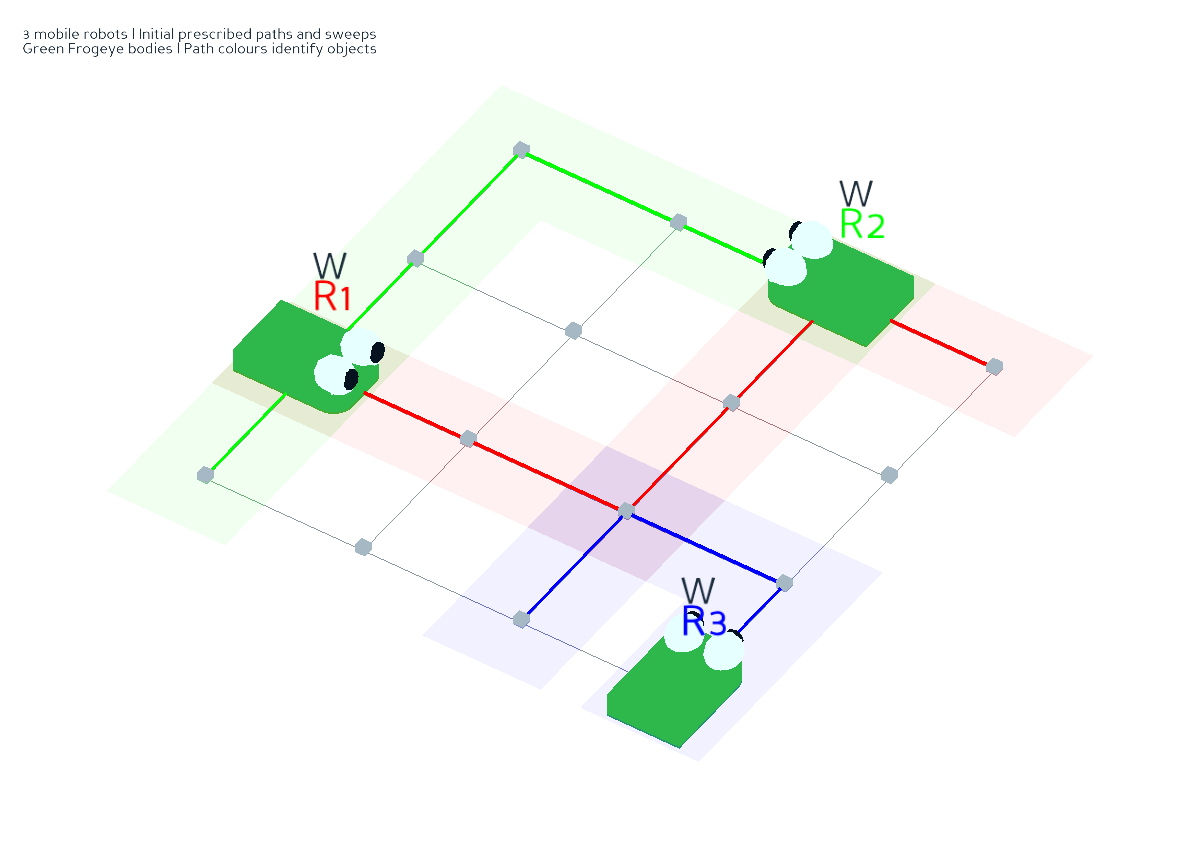
\includegraphics[width=\linewidth]{paper_03_04_RobotPath_SweepInterference.png}
\par\small (c) Transitive interference: 3 objects.\par\scriptsize $4\times4$, $K_I=6$, $L_I=15$~m.
\end{minipage}\hfill
\begin{minipage}{.48\linewidth}\centering
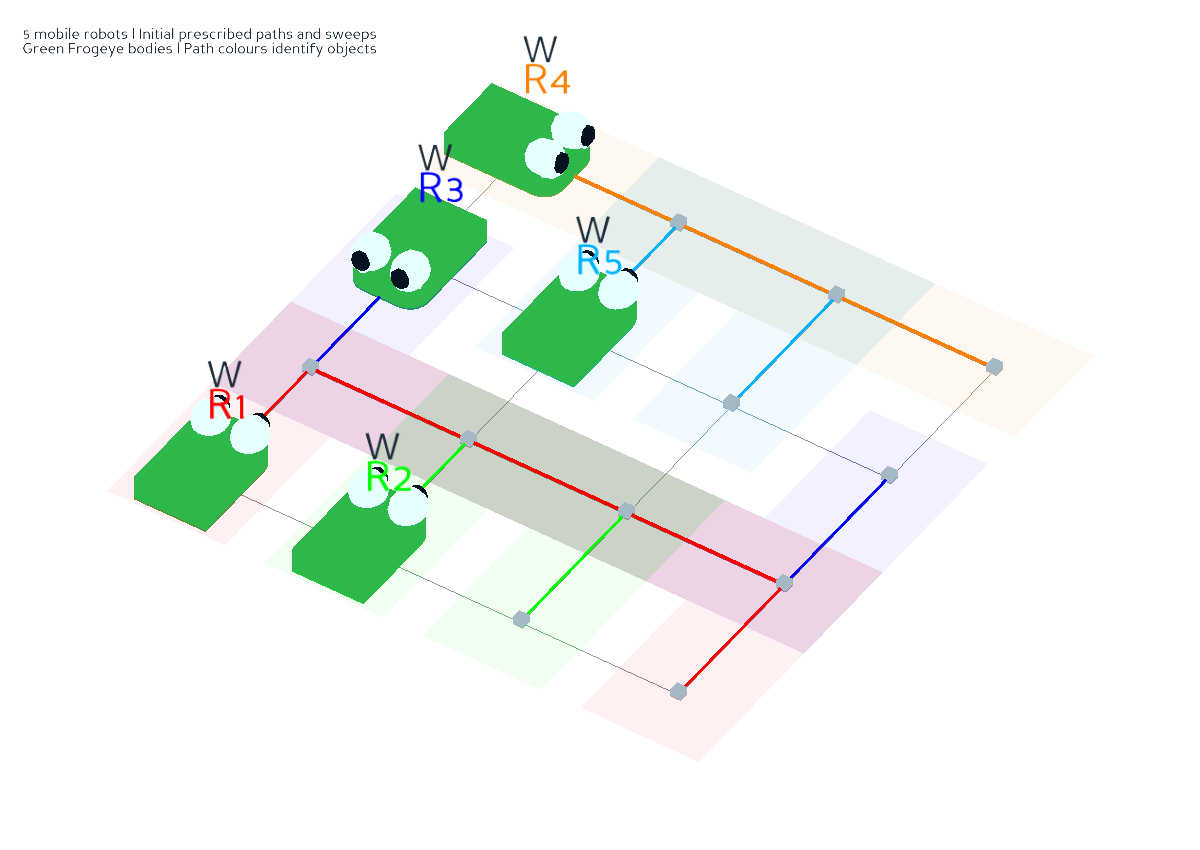
\includegraphics[width=\linewidth]{paper_05_01_RobotPath_TheoremSafeEndpoints.png}
\par\small (d) Multiple groups: 5 objects.\par\scriptsize $4\times4$, $K_I=8$, $L_I=48$~m.
\end{minipage}\par\medskip
\begin{minipage}{.48\linewidth}\centering
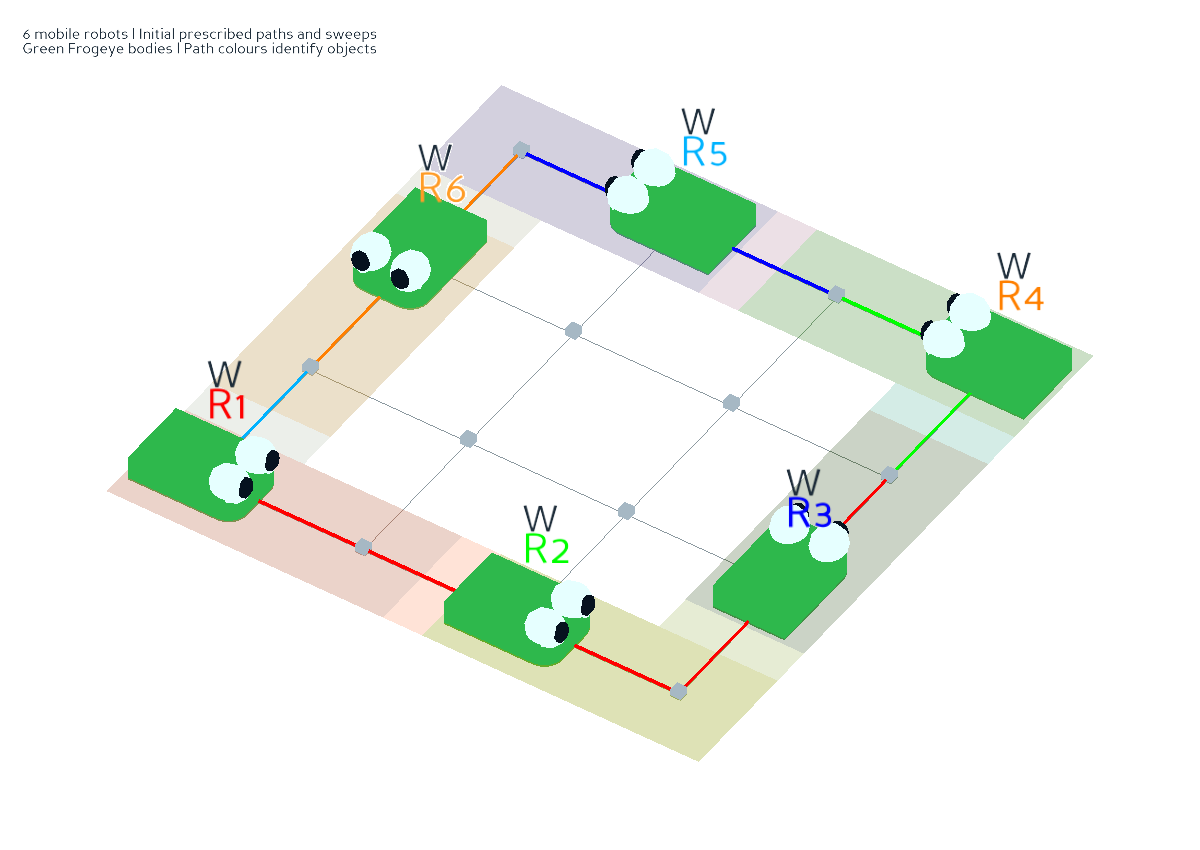
\includegraphics[width=\linewidth]{paper_06_01_RobotPath_Convoy.png}
\par\small (e) Perimeter convoy: 6 objects.\par\scriptsize $4\times4$, $K_I=24$, $L_I=132$~m.
\end{minipage}\hfill
\begin{minipage}{.48\linewidth}\centering
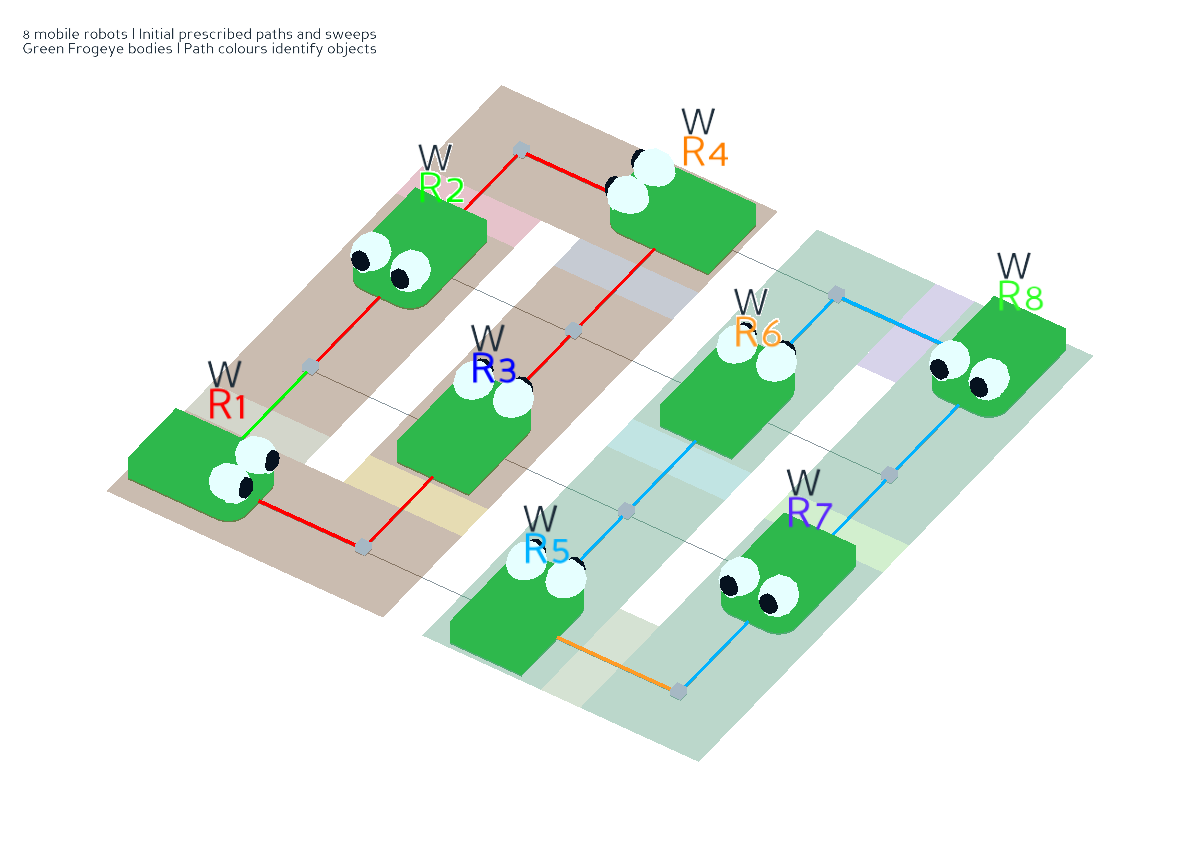
\includegraphics[width=\linewidth]{paper_08_02_RobotPath_InteriorTraffic.png}
\par\small (f) Interior mixed traffic: 8 objects.\par\scriptsize $4\times4$, $K_I=24$, $L_I=336$~m.
\end{minipage}\par\medskip
\caption{Actual Frogeye viewer captures defining the case types. Lines
and translucent sweeps show the given paths before motion; initial sweep
overlap is a coordination requirement, not an instantaneous collision.}
\label{fig:case-gallery}
\end{figure}
\begin{figure}[p]
\centering
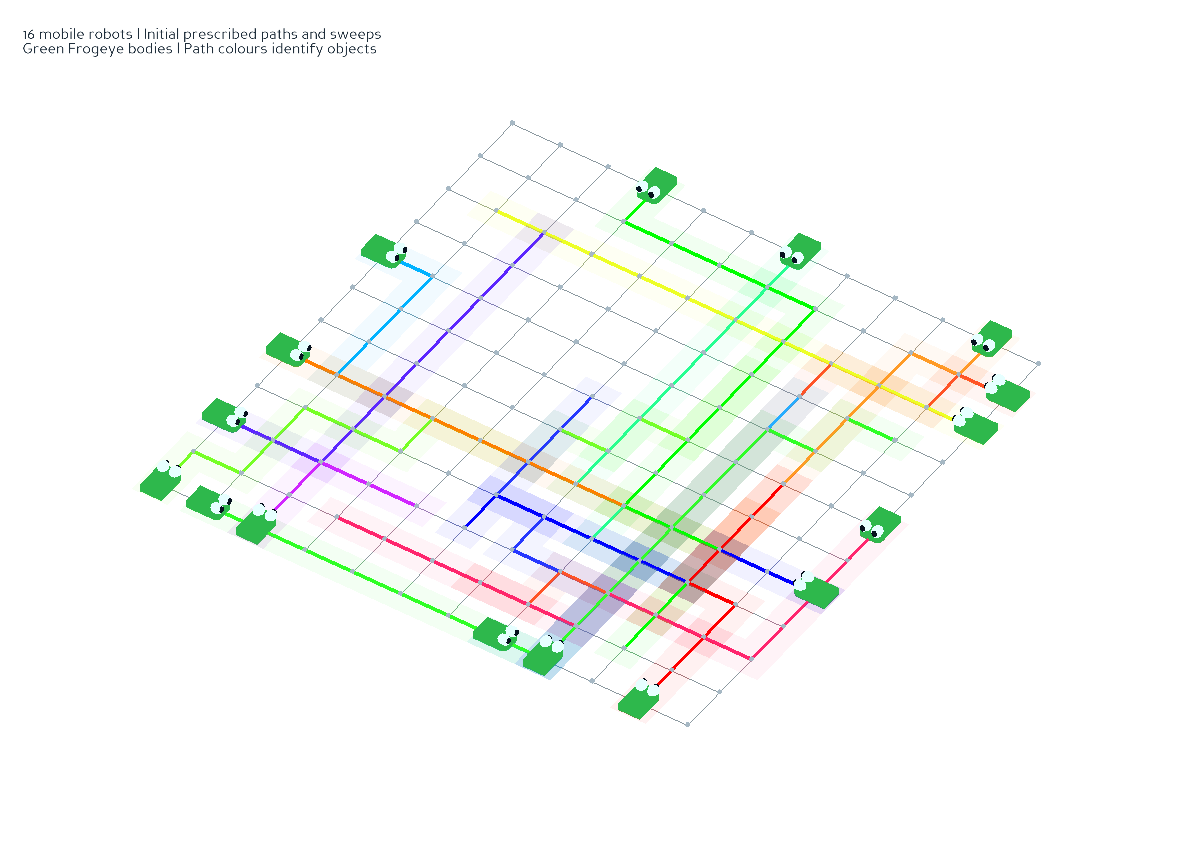
\includegraphics[width=.88\linewidth]{paper_generated_density16.png}
\par\small (a) Dense generated traffic: $12\times12$, 16 objects,
$K_I=130$, $L_I=580.0$~m.
\par\medskip
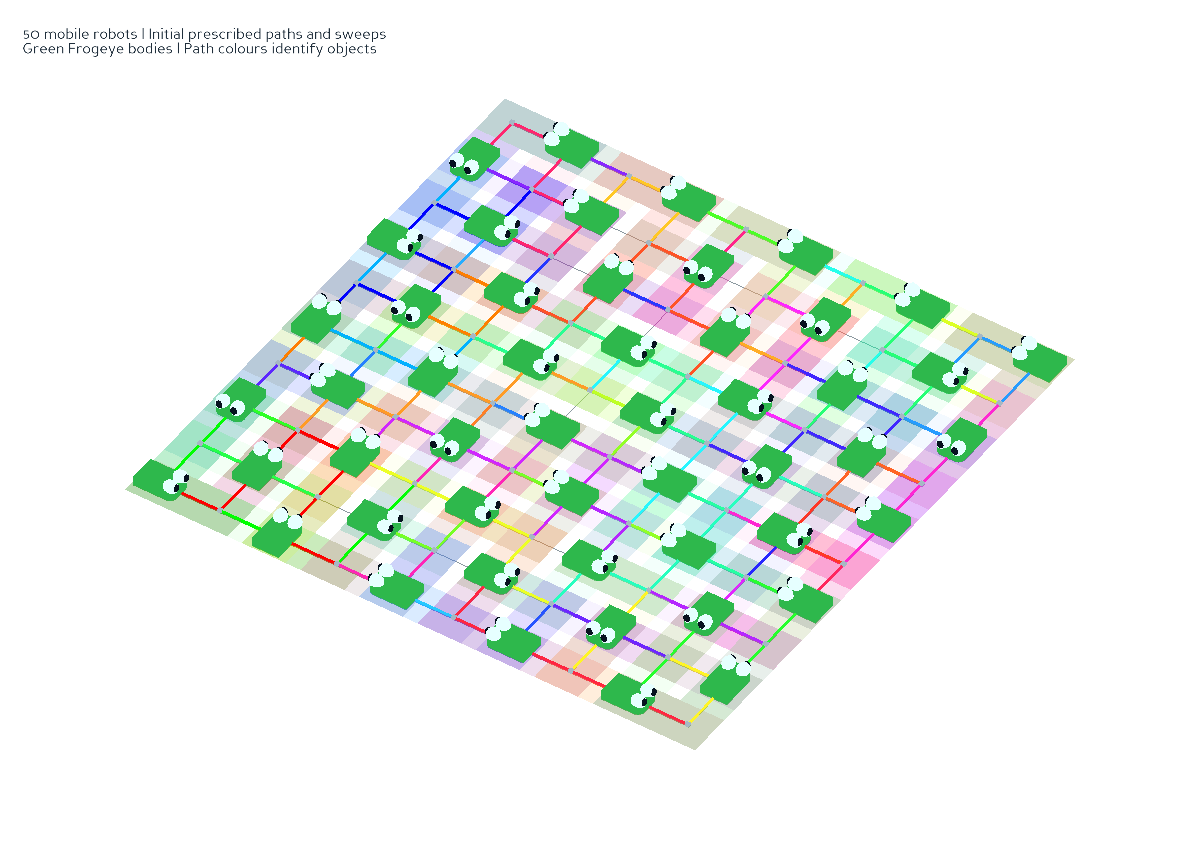
\includegraphics[width=.88\linewidth]{paper_50_01_RobotPath_InteriorTraffic.png}
\par\small (b) Interior mixed traffic: $10\times10$, 50 objects,
$K_I=631$, $L_I=2581.0$~m.
\caption{Complex fixed-path examples in the actual viewer. Captures show
initial states, not a claim of simultaneous execution of intersecting sweeps.
Completion is verified through the controlled executions in
Table~\ref{tab:stop-baseline-makespan}.}
\label{fig:dense-captures}
\end{figure}

\subsection{Execution and independent replay}
Each baseline case is executed with FIFO and LP as defined in
Section~\ref{sec:two-policies}. Main runs use DEVS events only, with
continuous and animation sampling intervals set to infinity. Each run is
then independently replayed with 0.1~s collision sampling and stopping
enabled for both MRobot and PSensor. A collision halts the Plant and counts
as a failed validation. Replay must match every issued command's identity,
owner and time, as well as the completion metrics.

Completion requires all original tasks finished, no active/awaiting command
or buffered output, every MRobot at its specified endpoint in Wait, every
PSensor in Idle, and a nonempty retained certificate set. Every command
must have exactly one approved--issued--arrived lifecycle. Thus engine
passivity alone is not counted as completion. The finite event budget is
a diagnostic limit, not an infeasibility test.

If object $i$ reaches its final endpoint at $C_i$, the reported measures are
\begin{equation}
 C_{\max}=\max_i C_i,\qquad \overline C=\frac1n\sum_i C_i.
 \label{eq:completion-measures}
\end{equation}
The post-fix measurements below replace the earlier validation-suite
performance table. Both policies use safe-prefix approach, per-point clearance
updates and sweep merging. Destination extension is disabled: every issued
command terminates at its approved endpoint before another movement starts.
The repaired same-time DEVS ordering delivers zero-time controller commands
first and resolves other simultaneous children by name. This removes object
identity as an experimental scheduling variable.

Thirteen fixed route sets are evaluated: two three-robot inspection cases,
three seeds each with 10, 20 and 30 robots, and two interior-traffic cases with
8 and 50 robots. Every FIFO/LP pair has identical paths, initial conditions and
validated certificate alternatives. LP uses both optional waiting for an
already-committed longer approach and longest-remaining-path selection among
eligible waiters; mandatory precedence and current occupancy are retained.
D10-19, for example, denotes the 10-robot DAG fixture with seed 20261119;
suffixes 20 and 21 denote seeds 20261120 and 20261121. Approach A and Braking B
identify the 03\_08 and 03\_09 routes, respectively, both run here with
extension disabled. Their nonuniform layouts have five coordinates per axis.

\IfFileExists{Data/stop_only_baseline_tables_20261121.tex}{%
% Generated from the post-fix stop-only measurements. Do not hand-edit numbers.
\begin{table}[htbp]
\centering\small
\setlength{\tabcolsep}{4pt}
\caption{Post-fix stop-only baseline: geometry and makespan in seconds. Both policies use safe-prefix approach and sweep merging; motion extension is OFF.}
\label{tab:stop-baseline-makespan}
\begin{tabular}{rlcrrrrr}
\toprule
ID & Case & Grid & $n$ & $K_I$ & $L_I$ (m) & FIFO $C_{\max}$ & LP $C_{\max}$\\
\midrule
1 & Approach A & $5\times5$ & 3 & 4 & 12.0 & 18.394 & 18.394\\
2 & Braking B & $5\times5$ & 3 & 4 & 12.0 & 25.372 & 25.372\\
3 & D10-19 & $10\times10$ & 10 & 70 & 253.0 & 115.847 & 115.847\\
4 & D10-20 & $10\times10$ & 10 & 42 & 170.5 & 83.082 & 83.082\\
5 & D10-21 & $10\times10$ & 10 & 66 & 262.5 & 117.809 & 117.809\\
6 & D20-19 & $10\times10$ & 20 & 238 & 993.5 & 245.375 & 251.998\\
7 & D20-20 & $10\times10$ & 20 & 226 & 1002.5 & 241.505 & 241.505\\
8 & D20-21 & $10\times10$ & 20 & 220 & 872.5 & 170.859 & 170.859\\
9 & D30-19 & $12\times12$ & 30 & 398 & 1703.5 & 293.672 & 275.788\\
10 & D30-20 & $12\times12$ & 30 & 326 & 1423.0 & 217.765 & 217.765\\
11 & D30-21 & $12\times12$ & 30 & 278 & 1230.5 & 142.185 & 142.185\\
12 & Interior & $4\times4$ & 8 & 24 & 336.0 & 42.921 & 42.921\\
13 & Interior & $10\times10$ & 50 & 631 & 2581.0 & 42.921 & 42.921\\
\bottomrule
\end{tabular}
\end{table}

\begin{table}[htbp]
\centering\small
\setlength{\tabcolsep}{4pt}
\caption{Post-fix stop-only baseline: mean and population standard deviation of final path-completion times, in seconds. IDs match Table~\ref{tab:stop-baseline-makespan}.}
\label{tab:stop-baseline-mean}
\begin{tabular}{rrrrr}
\toprule
ID & FIFO $\overline C$ & FIFO $\sigma_C$ & LP $\overline C$ & LP $\sigma_C$\\
\midrule
1 & 11.627 & 4.810 & 11.627 & 4.810\\
2 & 16.043 & 6.710 & 16.043 & 6.710\\
3 & 86.301 & 28.341 & 86.301 & 28.341\\
4 & 57.574 & 19.788 & 57.574 & 19.788\\
5 & 71.034 & 34.241 & 71.034 & 34.241\\
6 & 132.145 & 60.320 & 139.351 & 69.031\\
7 & 121.958 & 69.365 & 121.958 & 69.365\\
8 & 92.432 & 50.350 & 92.432 & 50.350\\
9 & 155.324 & 79.931 & 149.002 & 73.794\\
10 & 148.591 & 43.899 & 148.591 & 43.899\\
11 & 75.321 & 34.863 & 75.321 & 34.863\\
12 & 41.921 & 1.000 & 41.921 & 1.000\\
13 & 41.561 & 1.411 & 41.561 & 1.411\\
\bottomrule
\end{tabular}
\end{table}

\begin{table}[htbp]
\centering\small
\setlength{\tabcolsep}{4pt}
\caption{Stop-only execution cost and decisions. Wall time is the median of three DEVS-only runs, excluding model/certificate construction. Stops exclude final arrivals; LP holds and waiter arbitrations are counted per execution.}
\label{tab:stop-baseline-runtime}
\begin{tabular}{rrrrrrr}
\toprule
ID & FIFO (ms) & LP (ms) & FIFO stops & LP stops & LP holds & LP selections\\
\midrule
1 & 1.32 & 1.32 & 2 & 2 & 0 & 0\\
2 & 1.27 & 1.35 & 2 & 2 & 0 & 0\\
3 & 80.03 & 79.61 & 36 & 36 & 0 & 1\\
4 & 61.21 & 62.54 & 19 & 19 & 0 & 0\\
5 & 77.34 & 74.03 & 30 & 30 & 0 & 0\\
6 & 548.64 & 557.13 & 95 & 96 & 1 & 1\\
7 & 473.45 & 475.14 & 75 & 75 & 0 & 0\\
8 & 425.76 & 426.27 & 86 & 86 & 0 & 0\\
9 & 1925.18 & 1916.71 & 154 & 154 & 1 & 1\\
10 & 1741.28 & 1715.11 & 143 & 143 & 0 & 0\\
11 & 1286.06 & 1292.60 & 126 & 126 & 0 & 0\\
12 & 25.17 & 24.91 & 48 & 48 & 0 & 0\\
13 & 1511.99 & 1471.15 & 300 & 300 & 0 & 0\\
\bottomrule
\end{tabular}
\end{table}

}{%
% Generated from the post-fix stop-only measurements. Do not hand-edit numbers.
\begin{table}[htbp]
\centering\small
\setlength{\tabcolsep}{4pt}
\caption{Post-fix stop-only baseline: geometry and makespan in seconds. Both policies use safe-prefix approach and sweep merging; motion extension is OFF.}
\label{tab:stop-baseline-makespan}
\begin{tabular}{rlcrrrrr}
\toprule
ID & Case & Grid & $n$ & $K_I$ & $L_I$ (m) & FIFO $C_{\max}$ & LP $C_{\max}$\\
\midrule
1 & Approach A & $5\times5$ & 3 & 4 & 12.0 & 18.394 & 18.394\\
2 & Braking B & $5\times5$ & 3 & 4 & 12.0 & 25.372 & 25.372\\
3 & D10-19 & $10\times10$ & 10 & 70 & 253.0 & 115.847 & 115.847\\
4 & D10-20 & $10\times10$ & 10 & 42 & 170.5 & 83.082 & 83.082\\
5 & D10-21 & $10\times10$ & 10 & 66 & 262.5 & 117.809 & 117.809\\
6 & D20-19 & $10\times10$ & 20 & 238 & 993.5 & 245.375 & 251.998\\
7 & D20-20 & $10\times10$ & 20 & 226 & 1002.5 & 241.505 & 241.505\\
8 & D20-21 & $10\times10$ & 20 & 220 & 872.5 & 170.859 & 170.859\\
9 & D30-19 & $12\times12$ & 30 & 398 & 1703.5 & 293.672 & 275.788\\
10 & D30-20 & $12\times12$ & 30 & 326 & 1423.0 & 217.765 & 217.765\\
11 & D30-21 & $12\times12$ & 30 & 278 & 1230.5 & 142.185 & 142.185\\
12 & Interior & $4\times4$ & 8 & 24 & 336.0 & 42.921 & 42.921\\
13 & Interior & $10\times10$ & 50 & 631 & 2581.0 & 42.921 & 42.921\\
\bottomrule
\end{tabular}
\end{table}

\begin{table}[htbp]
\centering\small
\setlength{\tabcolsep}{4pt}
\caption{Post-fix stop-only baseline: mean and population standard deviation of final path-completion times, in seconds. IDs match Table~\ref{tab:stop-baseline-makespan}.}
\label{tab:stop-baseline-mean}
\begin{tabular}{rrrrr}
\toprule
ID & FIFO $\overline C$ & FIFO $\sigma_C$ & LP $\overline C$ & LP $\sigma_C$\\
\midrule
1 & 11.627 & 4.810 & 11.627 & 4.810\\
2 & 16.043 & 6.710 & 16.043 & 6.710\\
3 & 86.301 & 28.341 & 86.301 & 28.341\\
4 & 57.574 & 19.788 & 57.574 & 19.788\\
5 & 71.034 & 34.241 & 71.034 & 34.241\\
6 & 132.145 & 60.320 & 139.351 & 69.031\\
7 & 121.958 & 69.365 & 121.958 & 69.365\\
8 & 92.432 & 50.350 & 92.432 & 50.350\\
9 & 155.324 & 79.931 & 149.002 & 73.794\\
10 & 148.591 & 43.899 & 148.591 & 43.899\\
11 & 75.321 & 34.863 & 75.321 & 34.863\\
12 & 41.921 & 1.000 & 41.921 & 1.000\\
13 & 41.561 & 1.411 & 41.561 & 1.411\\
\bottomrule
\end{tabular}
\end{table}

\begin{table}[htbp]
\centering\small
\setlength{\tabcolsep}{4pt}
\caption{Stop-only execution cost and decisions. Wall time is the median of three DEVS-only runs, excluding model/certificate construction. Stops exclude final arrivals; LP holds and waiter arbitrations are counted per execution.}
\label{tab:stop-baseline-runtime}
\begin{tabular}{rrrrrrr}
\toprule
ID & FIFO (ms) & LP (ms) & FIFO stops & LP stops & LP holds & LP selections\\
\midrule
1 & 1.32 & 1.32 & 2 & 2 & 0 & 0\\
2 & 1.27 & 1.35 & 2 & 2 & 0 & 0\\
3 & 80.03 & 79.61 & 36 & 36 & 0 & 1\\
4 & 61.21 & 62.54 & 19 & 19 & 0 & 0\\
5 & 77.34 & 74.03 & 30 & 30 & 0 & 0\\
6 & 548.64 & 557.13 & 95 & 96 & 1 & 1\\
7 & 473.45 & 475.14 & 75 & 75 & 0 & 0\\
8 & 425.76 & 426.27 & 86 & 86 & 0 & 0\\
9 & 1925.18 & 1916.71 & 154 & 154 & 1 & 1\\
10 & 1741.28 & 1715.11 & 143 & 143 & 0 & 0\\
11 & 1286.06 & 1292.60 & 126 & 126 & 0 & 0\\
12 & 25.17 & 24.91 & 48 & 48 & 0 & 0\\
13 & 1511.99 & 1471.15 & 300 & 300 & 0 & 0\\
\bottomrule
\end{tabular}
\end{table}

}

\subsection{Outcome of the post-fix stop-only baseline}
The 13 route sets give 26 policy conditions, each repeated three times in
headless DEVS-only execution, followed by a separate 0.1-second
stop-on-collision replay. All 78 timed runs and 26 replays finish; replays
have zero detected contacts. Per-robot completion times and extension counters
are checked for repeatability. Every condition has zero extension commands.
Population standard deviations describe differences between robots within a
case, rather than uncertainty across repeated timings. The runtime table
reports medians of measured execution costs and excludes input/certificate
construction, rendering and collision replay.

LP has a lower makespan in one route set, a higher makespan in one, and ties
FIFO in eleven. The same direction of comparison holds for mean completion
time. These observations do not establish dominance of either policy. The
recorded LP holds occur twice; most cases do not present an optional
arrival-wait decision. A future efficiency comparison must rerun this frozen
stop-only baseline against the revised extension control. No efficiency gain
from destination extension is claimed from these baseline-only tables.

These results exercise the implemented certificate and occupancy guards;
completion guarantees depend on their stated assumptions. Successful cases
are implementation evidence, and sampled collision checking is not a
continuous-time proof.

\subsection{Application to a warehouse layout with twenty loaded robots}
\label{sec:warehouse}
The framework does not assume a regular grid of paths. This application
uses an aisle graph with 401 points and 527 bidirectional physical links,
nonuniform aisle spacing, ten workstations, and 120 rack cells. The present
geometric implementation still uses two-dimensional axis-aligned segments
and rectangular occupied envelopes; independence from a regular grid does
not imply an implemented arbitrary-geometry sweep engine.

Five fixed-path sets each contain twenty loaded robots. Ten depart from
rack cells toward the ten workstations, and ten depart from workstation
fronts toward return rack cells. Both groups carry racks. Twenty distinct
cells are vacated for these transfers, leaving 100 stationary racks.
Routes are generated before execution by distance-weighted A* on the aisle
graph, then checked for pairwise feasibility and an acyclic requirement
graph. These are fixed-path traffic experiments, not complete order cycles.
The robot chassis turns at corners while the rack orientation is held fixed
as an explicit RMFS modeling assumption.

\begin{figure}[p]
\centering
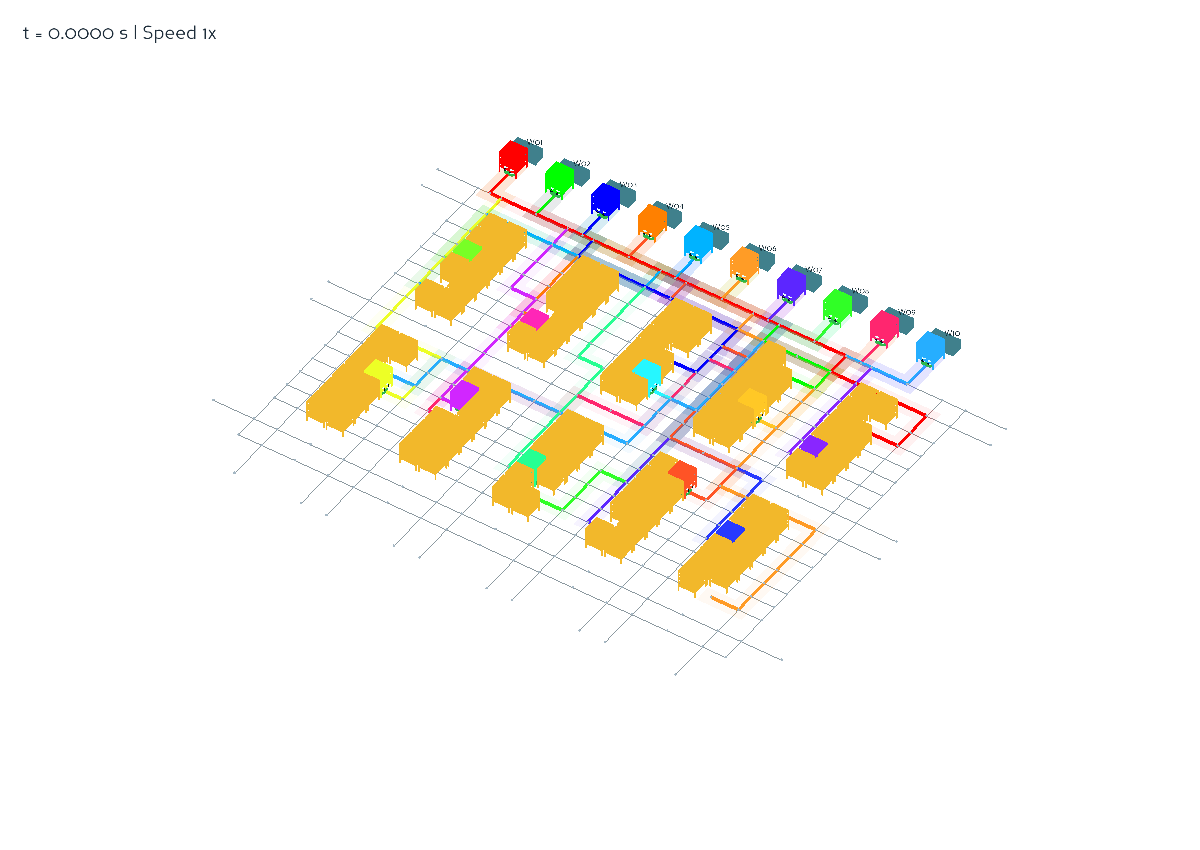
\includegraphics[width=.94\linewidth,trim=90 100 90 70,clip]{warehouse20_iso_initial.png}
\par\smallskip (a) Initial configuration and prescribed paths, $t=0$ s.
\par\medskip
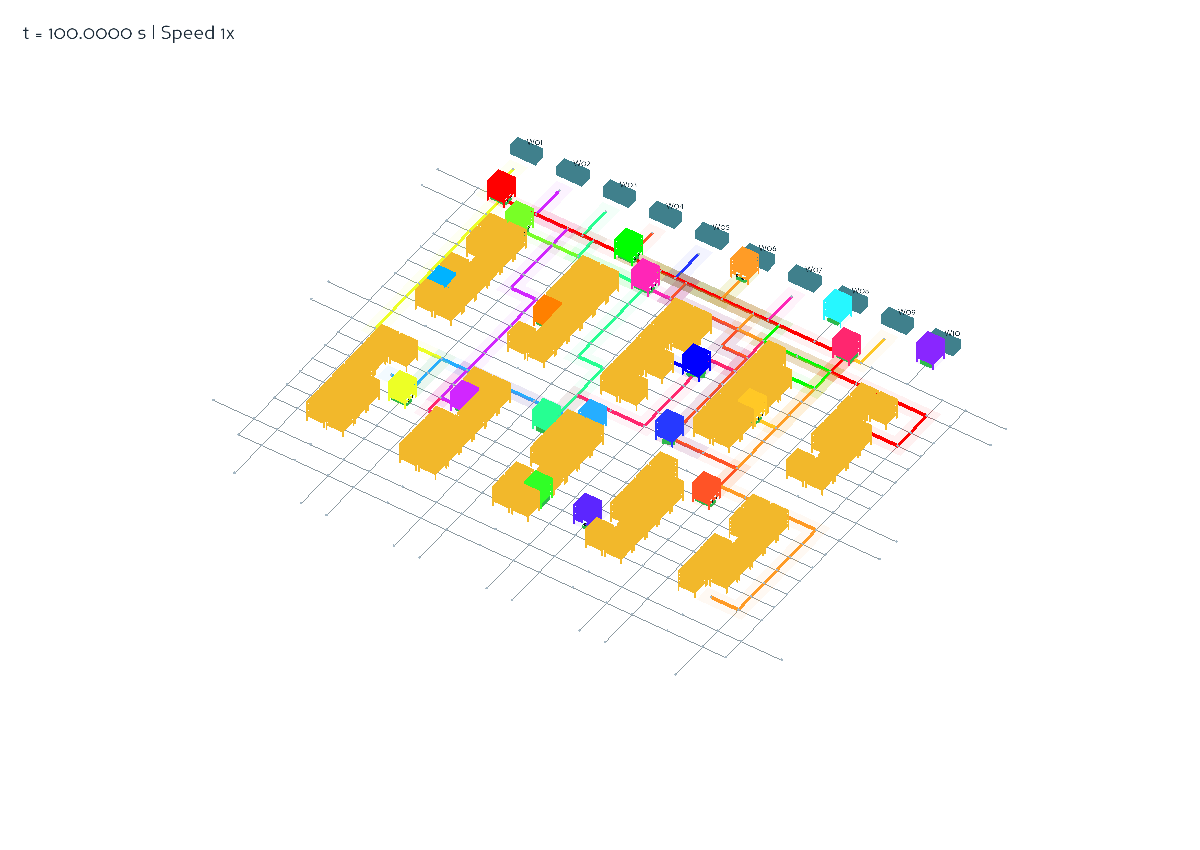
\includegraphics[width=.94\linewidth,trim=90 100 90 70,clip]{warehouse20_iso_progress.png}
\par\smallskip (b) FIFO execution and residual paths, $t=100$ s.
\caption{Actual Iso-view screenshots of warehouse set 1. Colored moving
racks correspond to twenty loaded robots; yellow racks remain stationary.
Reported physical progress releases passed path regions.}
\label{fig:warehouse-iso}
\end{figure}

\begin{table}[htbp]
\centering\small
\caption{Historical warehouse executions: twenty loaded robots on five fixed-path sets, not recollected in the current stop-only study.
All times are seconds. $K_I$ and $L_I$ use the same directed interference
interval definitions as Table~\ref{tab:stop-baseline-makespan}.}
\label{tab:warehouse-results}
\begin{tabular}{rrrrrrr}
\toprule
Set & $K_I$ & $L_I$ (m) & \multicolumn{2}{c}{FIFO} & \multicolumn{2}{c}{LP}\\
 & & & $C_{\max}$ & Mean & $C_{\max}$ & Mean\\
\midrule
1 & 252 & 1769.30 & 522.25 & 243.79 & 522.25 & 243.79\\
2 & 266 & 1756.48 & 413.24 & 216.81 & 413.24 & 216.81\\
3 & 310 & 2242.88 & 540.70 & 288.15 & 540.70 & 288.43\\
4 & 266 & 1696.35 & 359.65 & 197.50 & 359.65 & 197.50\\
5 & 256 & 1655.63 & 343.69 & 193.24 & 343.69 & 193.24\\
\bottomrule
\end{tabular}
\end{table}
All ten main executions completed, as did all ten independent replays
with collision stopping enabled and a 0.01 s validation interval. No robot
contacts were detected, and the replay command traces matched. Static
rack clearance was checked during route construction. FIFO and LP have
the same makespan in all five sets; only set 3 differs in mean completion
time. These results support completion and safe execution in this layout,
not a claim that LP improves makespan.

The experiment can be viewed using:
\begin{quote}\small\ttfamily
python -m examples.RMFS.Tests.20\_04\_RobotPath\_WarehouseExchange\\
\hspace*{1em}--case 1 --policy fifo --fps 10 --non-interactive
\end{quote}
\begin{sloppypar}
Choose cases 1--5 and policy \texttt{fifo} or \texttt{lp}. The results are
stored in \path{Tests/results/warehouse20_validation.json}; reproduce
validation with the module \path{examples.RMFS.Tests.run_warehouse_paths},
passing \texttt{--validate} to \texttt{python -m}.
That historical collection comprised 86 cases, 172 main runs and 172 replays.
It is retained for provenance; it is not the post-fix stop-only dataset.
\end{sloppypar}

\section{Assessment of results and industrial relevance}
\label{sec:contributions}

\paragraph{Novelty assessment after direct comparison.}
The correspondences in Section~\ref{sec:prior-art} change how these results
must be interpreted. Sweep compatibility, wait insertion, partial-progress
scheduling and precedence-based execution are established concepts.
Our definitions and proofs provide a specialized formulation and realization;
they are not claimed as the first general solution. In particular, the 1989
construction already treats endpoint blocking and schedules beyond
whole-path serialization, while SCALE supplies a broader integrated
planning/execution system. The following evidence documents the present
implementation, not a demonstrated theoretical or performance superiority.

\subsection{Geometry-based interference without a regular grid}
The framework defines conflicts through occupied-region sweeps, not cell
identity. Nonuniform spacing and a general path graph therefore require no
change to the abstract tuple and execution conditions. The warehouse
experiment in Section~\ref{sec:warehouse} demonstrates this separation on
401 points and 527 bidirectional links. Its paths remain axis-aligned;
arbitrary curved paths and general 3D sweeps are not implemented.

The distinction from cell-based planning is useful where rack dimensions,
clearance and aisle geometry do not coincide with a regular cell partition.
It does not remove the need for a safe geometric envelope. Nor is non-grid
coordination itself new: the earlier geometric methods reviewed in
Section~2 already provide it.

\begin{table}[htbp]
\centering\small
\caption{Established capabilities and the present realization. Differences
in representation are not themselves novelty claims.}
\label{tab:literature-comparison}
\begin{tabular}{p{.22\linewidth}p{.34\linewidth}p{.35\linewidth}}
\toprule
Issue & Prior approach & Present approach\\
\midrule
Conflict representation & Segment-sweep conflicts~\cite{odonnell1989};
geometric coordination~\cite{leroy1999}; heterogeneous sweeps~\cite{scale2026}
& Fixed rectangular sweeps; no regular-grid premise, also present in prior work.\\[4pt]
Schedule construction & Segment-progress search and endpoint blocking~\cite{odonnell1989}
& Point-token/wait search, with the finite correspondence in
Equation~\eqref{eq:prior-progress}.\\[4pt]
Geometric cost & Coordination diagrams~\cite{leroy1999}; adaptive
clearance queries~\cite{ablad2021} & Rectangular segment sweeps in the
current 2D implementation.\\[4pt]
Execution & Priority and dependency-based safe
execution and action combination~\cite{gregoire2015,cap2016,hoenig2019,berndt2024,scale2026} & Validated tuples,
original-task order, permitted merging and reported residual release.\\[4pt]
Demonstration & Different geometries, fleet sizes and workloads &
Post-fix: 13 route sets under FIFO/LP, up to 50 robots. Historical warehouse
and illustrative executions are retained separately.\\
\bottomrule
\end{tabular}
\end{table}

\subsection{A computationally tractable realization of sweep control}
Our implementation addresses sweep cost by choosing a simple occupied
shape and motion class, then releasing passed regions on meaningful
reports. Rectangular sweeps are exact for the selected fixed-orientation
rectangular model, while that model approximates physical robots and
loads. The controller avoids repeated fixed-time departure checks;
acceleration, cruising, braking and rotation are scheduled in the timed
DEVS Plant. Original movement tasks remain available for approval even
when several are merged into one continuous command.

\paragraph{Timed execution with interactive animation.}
The implemented demonstration couples event-driven traffic control to a
3D animated Plant with acceleration, constant-speed travel, deceleration,
and rotation. At the $1\times$ setting, the viewer targets real-time-paced
playback while the simulated controller continues to process clearance and
arrival events. This exposes the connection between untimed passage order
and timed physical motion, rather than displaying only a final plan.
Iso screenshots of the warehouse application are shown in
Figure~\ref{fig:warehouse-iso}. Animation and DEVS execution use the same
model; screen sampling does not impose a fixed-time control loop.
The 50-robot display was visibly affected by rendering load, so no measured
frame-rate or real-time deadline guarantee is inferred from this demonstration.

\paragraph{Simulation computation time.}
Table~\ref{tab:realtime-evidence} reports the recorded headless 50-robot
runs. Both simulate 42.92 s in less than 10 s of wall-clock time, including
model setup: approximately 4.5 times faster than real time on the experiment
machine. Route generation and external workload preparation precede these
measurements; rendering and the separate sampled collision replay are
excluded. Thus the data demonstrate timed simulation computation faster than real time
for this case. These timings do not measure the animated run; rendering has
a separate cost.

\begin{table}[htbp]
\centering\small
\caption{Historical timing of the 50-robot interior-traffic case before the latest fixes; the fresh execution-only medians are in Table~\ref{tab:stop-baseline-runtime}.
Values are individual recorded runs, not repeated-run averages. Wall time
includes model setup; no rendering or sampled collision checks are active.}
\label{tab:realtime-evidence}
\begin{tabular}{lrrrr}
\toprule
Policy & Simulated time (s) & Setup (s) & Total wall time (s) & Sim./wall\\
\midrule
FIFO & 42.92 & 1.15 & 9.62 & 4.46\\
LP   & 42.92 & 1.12 & 9.56 & 4.49\\
\bottomrule
\end{tabular}
\end{table}
This establishes feasibility for the reported inputs. It is not a scaling
law or a speed comparison with older papers on different hardware and
workloads. In particular, fleet size alone does not measure difficulty:
interference count, total interference length and interaction connectivity
also matter.

\subsection{Contribution to RMFS modeling and control}
The significance of this work has two parts. First, the established sweep
and ordering properties make it possible to construct and execute
collision-free control for given paths satisfying the stated completion
conditions. Point waits and permitted merging translate these properties
into executable commands without losing the required interference order.
The proof states the assumptions. The post-fix study verifies 13 route sets
under FIFO and LP, with three timed repeats and an independent collision-stop
replay per policy; earlier warehouse and illustrative records are labelled historical.

Second, these results establish a foundation for interference-aware optimal
path generation. A candidate route can be evaluated against the robots'
residual sweeps and the completion conditions, rather than selected solely
by its isolated geometric length. RobotPathPlanner can build on this
control layer to compare feasible routes by a specified time-based
objective. The generation and optimization algorithm, and its evaluation,
will be presented in a subsequent study; optimal path generation is not
claimed as a result of the present paper.

For RMFS engineering, this supplies inspectable reservations, meaningful
clearance feedback and reproducible tests on rack-carrying robots. A cell
layout may be used, but is not required by the framework. Remaining work
is to generate admissible routes to changing destinations; the present
results concern completion of supplied paths. Real deployment additionally
requires envelopes and feedback margins that cover localization error,
communication delay and stopping uncertainty.

\section{Reproducibility and limitations}
\label{sec:reproducibility}

\subsection{Repository and reader access}
The source repository is
\begin{center}
\url{https://github.com/mhhwang2002/SOCS}.
\end{center}
All paths below are relative to its root directory. The implementation and
examples are in \nolinkurl{examples/RMFS}; unit tests are in
\nolinkurl{tests/examples/RMFS}. The manuscript source is
\nolinkurl{docs/RMFS/Papers/2026_11_SweepBasedCollisionAvoidanceFramework/}\allowbreak
\nolinkurl{SweepBasedCollisionAvoidanceFramework_en.tex}.

For unrestricted reader access, the repository or a reproducibility mirror
must be publicly readable. A public GitHub repository can be viewed and
cloned without granting readers write permission. A private repository
requires explicit access for each reader. This manuscript does not assert
that visibility has already been changed.\footnote{GitHub's visibility
model is documented at
\url{https://docs.github.com/en/repositories/creating-and-managing-repositories/about-repositories}.}
The newly added artifacts must be committed and pushed before readers can
fetch them. Before publication, the authors should cite an immutable commit
or release tag containing the code and data; no release identifier has yet
been frozen for this working draft.

\subsection{Environment setup}
The package requires Python 3.13 or later. Panda3D provides animation;
the development extra installs pytest for regression tests. From a checkout,
create and activate a virtual environment, then install the package in
editable mode:
\begin{quote}\small
\begin{verbatim}
git clone https://github.com/mhhwang2002/SOCS.git
cd SOCS
python -m venv .venv
\end{verbatim}
\end{quote}
On Windows PowerShell, activate it with
\begin{quote}\small
\begin{verbatim}
.\.venv\Scripts\Activate.ps1
\end{verbatim}
\end{quote}
On macOS/Linux, the equivalent activation command is
\begin{quote}\small
\begin{verbatim}
source .venv/bin/activate
\end{verbatim}
\end{quote}
Use \nolinkurl{python3} to create the environment if that is the available
Python command. With the environment active, run
\begin{quote}\small
\begin{verbatim}
python -m pip install -e ".[dev]" panda3d
\end{verbatim}
\end{quote}
The reported experiments were executed on Windows. The alternative shell
activation command does not constitute validation of every example on other
operating systems. Run all commands below from the repository root.

\subsection{Running and reproducing the reported cases}
The current post-fix baseline is reproduced from the repository root with:
\begin{quote}\small\begin{verbatim}
python -m examples.RMFS.Tests.run_release_extension_comparison --stop-only
python -m examples.RMFS.Tests.write_stop_baseline_tables
\end{verbatim}\end{quote}
The first command runs only approved-destination stopping, with FIFO and LP,
three headless repetitions, and 0.1-second stop-on-collision validation.
The second generates the manuscript tables directly from
\nolinkurl{examples/RMFS/Tests/results/stop_only_baseline_20261121.json}.
A CSV with per-case metrics is stored beside it. The JSON retains paths,
input fingerprints, source hashes, individual execution times, completion
times and validation status. Historical records such as
\nolinkurl{paper_fifo_lp_final.json} do not supply the new baseline tables.

The path data are under
\nolinkurl{examples/RMFS/Tests/data/generated/}. The \texttt{density12}
subdirectory contains \texttt{objects\_4.json}, \texttt{objects\_8.json},
\texttt{objects\_12.json} and \texttt{objects\_16.json}; \texttt{complex.json}
and \texttt{random\_trial.json} contain the other generated families.
Each file stores its seed, generator arguments, geometry, endpoint checks
and validated witness. \nolinkurl{generate_path_data}, with \texttt{--help}, lists the
generation parameters. Acceptance never uses completion-time performance.

Actual viewer captures are produced by
\nolinkurl{examples/RMFS/Tests/capture_paper_examples.py}. For example:
\begin{quote}\small\begin{verbatim}
python -m examples.RMFS.Tests.capture_paper_examples `
  --case 03_04_RobotPath_SweepInterference `
  --output three_objects.png
\end{verbatim}\end{quote}
Backticks are PowerShell line continuations; join the lines for other shells.
This captures the actual initial viewer state, not a synthetic drawing.
Original scenario modules illustrate prescribed routes; files whose names
contain \texttt{NoControl} or \texttt{Collision} retain their historical
uncontrolled demonstrations. Those names do not describe the controlled
numerical runs in this paper.

For the controlled two- and three-object animations, the existing launcher
\par\noindent\nolinkurl{run_framework_paper_examples}\par\noindent with \texttt{--case 2} or \texttt{--case 3}
uses the original single-reference controller. It illustrates execution of
the same geometry, whereas the two-policy numerical results are reproduced
with the validation command above. In the viewer, \textbf{A} toggles
automatic/manual mode, \textbf{Space} advances an event, \textbf{R} resets,
\textbf{T/I} select Top/Iso, \textbf{U/D} change speed, and \textbf{Esc}
closes. The default background is white.

The finite endpoint classification is reproduced with:
\begin{quote}\small\begin{verbatim}
python -m examples.RMFS.Tests.run_unit_pair_classification --max-edges 5
\end{verbatim}\end{quote}
This is the restricted finite classification, not a claim of general
necessary-and-sufficient feasibility for arbitrary paths.
The focused policy-definition and feedback tests are under
\nolinkurl{tests/examples/RMFS}:
\begin{quote}\small
\nolinkurl{test_paper_policy_definition.py}\par
\nolinkurl{test_fifo_traffic.py}\par
\nolinkurl{test_event_release.py}
\end{quote}

\subsection{Limitations}

The principal limitations are:
\begin{enumerate}
\item The task-based correctness argument is a proof sketch under explicit
      Plant and feedback assumptions; a formal verification of the numerical
      implementation is not provided.
\item Static acyclic requirements reject some feasible cyclic situations.
\item Safety margins, communication delay, localization errors, unexpected
      obstacles, and physical stopping behavior require further treatment.
\item The finite classification and performance studies do not establish
      general completeness, capacity, or optimality.
\item The relationship to prior methods needs a deeper technical comparison
      before claiming a new coordination result.
\end{enumerate}

\section{Conclusion and scope of subsequent work}
The paper links established sweep-based coordination principles to an event-driven
implementation of controlled motion. Complete tuple paths represent
movement and waiting, safe merging retains original control units, and
conservative release updates the shared RoadMap. The stated propositions
establish safety and finite completion under explicit geometric, feedback
and execution assumptions. FIFO and LP choose among permitted actions;
their preferences do not replace those safety or completion conditions.
The region-based formulation is general, while the implemented geometry
and the numerical evidence in this paper are restricted to the two-dimensional
rectangular-envelope mobile-robot model.

The current stop-only baseline completed 13 route sets under both policies,
with three timed repetitions and a matching independent collision-stop
replay per condition. It ranges from three-robot inspection cases to
50-robot interior traffic,
and reports interference count and total interference length beside the
completion measures. This is implementation-level confirmation of the
theory on the reported cases, rather than an empirical substitute for its
proof or a claim covering every physical disturbance.

The demonstrated engineering result is property-based, collision-free control of
given paths under the stated completion conditions. Its further significance
is the foundation it provides for \emph{interference-aware optimal path
generation}. Given current robot positions, destinations and residual
sweeps, RobotPathPlanner can use the derived conditions to assess candidate
routes and use the timed execution model to evaluate a specified
completion-time objective. A subsequent study will develop and evaluate
this path-generation and optimization method. The present paper establishes
the control foundation on which that study will build.

\paragraph{Future work: time-aware traffic admission and safe order repair.}
A separate required follow-up is to apply and evaluate the time-based
passage-order repair of Coskun and O'Kane~\cite{coskun2019}, together with
the Segment Graph deadlock checks~\cite{coskun2021}, in our TrafficManager.
Residual sweeps may intersect even when a robot can clear the shared region
before another can enter it. The present conservative controller can therefore
impose avoidable waiting. Future work must estimate clearance and arrival
times from the acceleration, braking and rotation model, test proposed order
changes against global dependencies and persistent endpoint occupancy,
record reservations consistently, and retain actual Plant clearance feedback.
Expected times alone are not safety certificates. Comparison with the current
controller should measure unnecessary waiting, completion time, computation
cost, collisions and deadlocks, including delay and downstream-blocking cases.
The application of these techniques and its guarantees are not results
established by the experiments reported in this paper.

Decision timing is a specific follow-up variable: compare a stopped-state
lookahead with a moving-state lookahead triggered just before braking would
begin. Section~\ref{sec:prebraking-review} separates direct precedents for
braking-boundary events, simulation-based entry permission and brake-line
stop/go control. The proposed experiment must not describe those established
components as absent from prior work.

The direct literature comparison does not establish a new general feasibility
or execution principle. The two-robot finite construction corresponds to
classical segment-progress coordination, and existing action graphs can
represent the examined alternating-progress witness. SCALE covers broader
integrated planning and execution functions. These findings should be retained
even if no independent theoretical contribution ultimately remains: the
implementation is a reproducible research foundation, and a future routing
method must be evaluated on its own evidence rather than inheriting a novelty
claim from the present terminology or simulator.

This paper closes with fixed-path collision avoidance and completion under the
stated assumptions. A separate study will compare stop-first admission with
Push/Pull control, using a pre-braking request and verified release to extend a
moving robot's profile. It will evaluate fleet battery energy and makespan on
matched routes and traffic orders, with robot, rack, and payload masses modeled
separately. Energy savings and joint optimization are objectives of that study.

% The reviewed reference list is shared in content with the separate residual
% decomposition draft. Bibliography follows inline for simple XeLaTeX builds.
\begin{thebibliography}{99}

\bibitem{zeigler1976}
B.~P. Zeigler.
\newblock \emph{Theory of Modelling and Simulation}.
\newblock First edition. Wiley-Interscience, New York, 1976.

\bibitem{zeigler2018}
B.~P. Zeigler, A. Muzy, and E. Kofman.
\newblock \emph{Theory of Modeling and Simulation: Discrete Event \& Iterative
System Computational Foundations}.
\newblock Third edition. Academic Press, 2018.
\newblock \url{https://doi.org/10.1016/C2016-0-03987-6}.

\bibitem{odonnell1989}
P.~A. O'Donnell and T. Lozano-P\'erez.
\newblock Deadlock-free and collision-free coordination of two robot manipulators.
\newblock In \emph{Proceedings of the IEEE International Conference on Robotics
and Automation}, pp.~484--489, 1989.
\newblock \url{https://lis.csail.mit.edu/pubs/tlp/coordination-o-donnell.pdf}.

\bibitem{leroy1999}
S. Leroy, J.-P. Laumond, and T. Sim\'eon.
\newblock Multiple path coordination for mobile robots: A geometric algorithm.
\newblock In \emph{Proceedings of the Sixteenth International Joint Conference
on Artificial Intelligence}, pp.~1118--1123, 1999.
\newblock \url{https://ijcai.org/proceedings/1999/0159.pdf}.

\bibitem{standley2011}
T.~S. Standley and R.~E. Korf.
\newblock Complete algorithms for cooperative pathfinding problems.
\newblock In \emph{Proceedings of the Twenty-Second International Joint
Conference on Artificial Intelligence}, pp.~668--672, 2011.
\newblock \url{https://doi.org/10.5591/978-1-57735-516-8/IJCAI11-118}.

\bibitem{gregoire2015}
J. Gregoire, S. Bonnabel, and A. de La Fortelle.
\newblock Robust multirobot coordination using priority encoded homotopic constraints.
\newblock arXiv:1306.0785v3, 2015. First submitted in 2013.
\newblock \url{https://arxiv.org/abs/1306.0785v3}.

\bibitem{cap2016}
M. \v{C}\'ap, J. Gregoire, and E. Frazzoli.
\newblock Provably safe and deadlock-free execution of multi-robot plans under
delaying disturbances.
\newblock arXiv:1603.08582, 2016.
\newblock \url{https://arxiv.org/abs/1603.08582}.

\bibitem{hoenig2019}
W. H\"onig, S. Kiesel, A. Tinka, J.~W. Durham, and N. Ayanian.
\newblock Persistent and robust execution of MAPF schedules in warehouses.
\newblock \emph{IEEE Robotics and Automation Letters}, 4(2):1125--1131, 2019.
\newblock \url{https://whoenig.github.io/publications/2019_RA-L_Hoenig.pdf}.

\bibitem{ablad2021}
E. {\AA}blad, D. Spensieri, R. Bohlin, and A.-B. Str\"omberg.
\newblock Continuous collision detection of pairs of robot motions under velocity uncertainty.
\newblock \emph{IEEE Transactions on Robotics}, 37(5):1780--1791, 2021.
\newblock \url{https://doi.org/10.1109/TRO.2021.3050011}.

\bibitem{coskun2021}
A. Coskun, J.~M. O'Kane, and M. Valtorta.
\newblock Deadlock-free online plan repair in multi-robot coordination with disturbances.
\newblock In \emph{FLAIRS}, 2021.
\newblock \url{https://jokane.net/pubs/CosOKaVal21.pdf}.

\bibitem{coskun2019}
A. Coskun and J.~M. O'Kane.
\newblock Online plan repair in multi-robot coordination with disturbances.
\newblock In \emph{IEEE International Conference on Robotics and Automation},
pp.~3333--3339, 2019.
\newblock \url{https://jokane.net/pubs/CosOKa19.pdf}.

\bibitem{dresner2008}
K. Dresner and P. Stone.
\newblock A multiagent approach to autonomous intersection management.
\newblock \emph{Journal of Artificial Intelligence Research}, 31:591--656, 2008.
\newblock \url{https://doi.org/10.1613/jair.2502}.
\newblock Author copy: \url{https://www.cs.utexas.edu/~pstone/Papers/bib2html-links/JAIR08-dresner.pdf}.

\bibitem{quesel2016}
J.-D. Quesel, S. Mitsch, S. Loos, N. Ar\'echiga, and A. Platzer.
\newblock How to model and prove hybrid systems with KeYmaera: a tutorial on safety.
\newblock \emph{International Journal on Software Tools for Technology Transfer},
18:67--91, 2016. Published online in 2015.
\newblock \url{https://doi.org/10.1007/s10009-015-0367-0}.

\bibitem{kalose2024}
A. Kalose, D. Willemsen, and J. Brouwer.
\newblock Human centric intersection crossing control using C-ITS information.
\newblock In \emph{VEHITS}, pp.~284--292, 2024.
\newblock \url{https://doi.org/10.5220/0012623500003702}.

\bibitem{berndt2024}
A. Berndt, N. van Duijkeren, L. Palmieri, A. Kleiner, and T. Keviczky.
\newblock Receding horizon re-ordering of multi-agent execution schedules.
\newblock \emph{IEEE Transactions on Robotics}, 40:1356--1372, 2024.
\newblock \url{https://doi.org/10.1109/TRO.2023.3344051}.

\bibitem{scale2026}
B. Cao.
\newblock From real-time planning to reliable execution: Scalable coordination
for heterogeneous multi-robot fleets in industrial environments.
\newblock arXiv:2607.00591v2, July 3, 2026. Reviewed manuscript;
no journal publication status is inferred here.
\newblock \url{https://arxiv.org/abs/2607.00591v2}.

\bibitem{li2021}
J. Li, A. Tinka, S. Kiesel, J. W. Durham, T. K. S. Kumar, and S. Koenig.
\newblock Lifelong multi-agent path finding in large-scale warehouses.
\newblock In \emph{Proceedings of the AAAI Conference on Artificial Intelligence},
35(13):11272--11281, 2021.
\newblock \url{https://publications.ri.cmu.edu/lifelong-multi-agent-path-finding-in-large-scale-warehouses}.

\bibitem{mir600guide}
Mobile Industrial Robots.
\newblock \emph{MiR600 User Guide (en)}, version 1.1, October 2021.
\newblock Sections 9.3--9.4, pp.~79--81.
\newblock Manufacturer document, distributor-hosted copy:
\url{https://noll-sondermaschinenbau.de/downloads/downloads_fts/mir600_user_guide_1.1_en.pdf}.

\bibitem{mir600}
Mobile Industrial Robots.
\newblock MiR600 Specifications.
\newblock \url{https://mobile-industrial-robots.com/products/robots/mir600/specifications}.
\newblock Accessed November 20, 2026.

\end{thebibliography}

\clearpage
\appendix
\section{DEVS Models of MRobot and PSensor}
\label{app:plant-models}
Each physical robot is represented by one MRobot and one PSensor atomic
DEVS model. Figure~\ref{fig:mrobot-phases} shows command execution;
Figure~\ref{fig:psensor-phases} shows event-based clearance sensing.
An edge label has the form [guard or input] / action and outputs.
Internal edges occur when the source phase's time advance expires.

\subsection{MRobot: acceleration, travel, and deceleration}
For a positive stop-to-stop straight distance $D$, acceleration $a$, deceleration
$b$, and speed limit $v$, the profile peak speed and duration are
\begin{equation}
 v_p=\min\!\left(v,\sqrt{\frac{2D}{1/a+1/b}}\right),\qquad
 T(D)=\frac{D}{v_p}+\frac{v_p}{2}\left(\frac1a+\frac1b\right).
 \label{eq:profile}
\end{equation}
This includes triangular and trapezoidal profiles. Current empty-robot
parameters are $a=b=0.41\,\mathrm{m/s^2}$, $v=2\,\mathrm{m/s}$, and yaw rate
$45\,\mathrm{deg/s}$. Loaded parameters use $a=b=0.37\,\mathrm{m/s^2}$ and
yaw rate $30\,\mathrm{deg/s}$, with the same speed limit. These are simulation
parameters inherited from the earlier example; braking and yaw values are
model assumptions, not newly verified manufacturer specifications.


MRobot approximates MiR600 motion with the triangular or trapezoidal
velocity profile in Equation~\eqref{eq:profile}. Short moves accelerate and
then decelerate; sufficiently long moves also contain a constant-speed
interval. Collinear intermediate points do not force a stop. A change of
heading invokes RotateTo, while the rack's orientation remains fixed in
this RMFS model. The speed limit follows the published MiR600
specification~\cite{mir600}; equal braking and acceleration magnitudes and
the yaw rates are simulation assumptions, not a manufacturer-validated
dynamic identification.

\begin{figure}[htbp]
\centering
\resizebox{0.98\linewidth}{!}{%
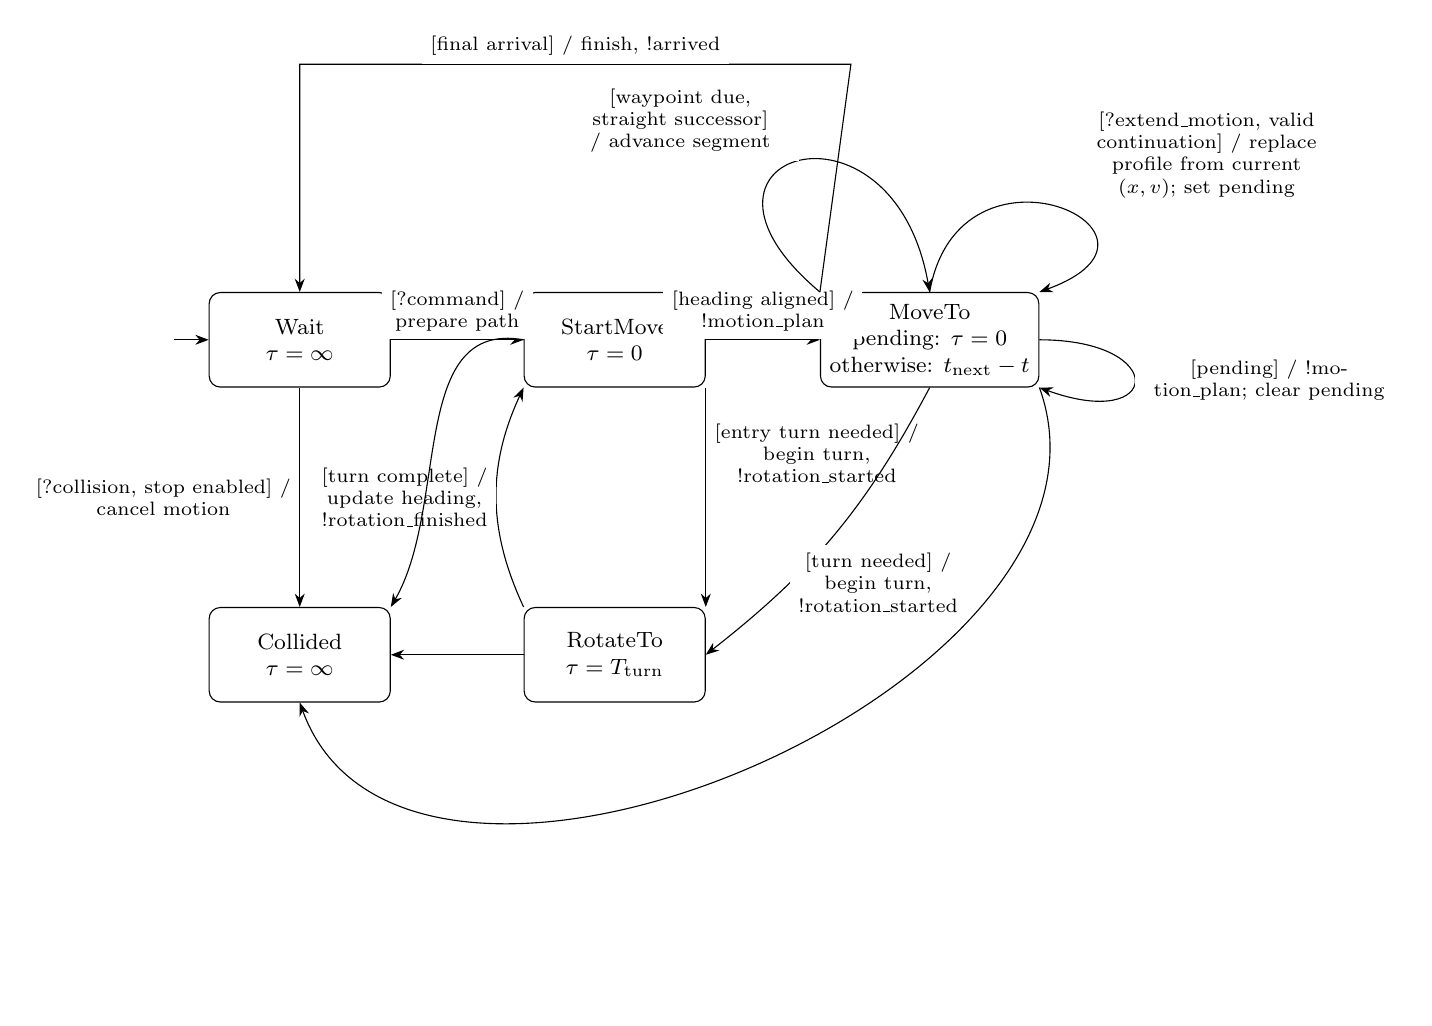
\begin{tikzpicture}[>=Stealth,every node/.style={font=\footnotesize},
 phase/.style={draw,rounded corners,align=center,minimum width=23mm,minimum height=12mm},
 lab/.style={align=center,fill=white,inner sep=3pt,font=\scriptsize}]
\node[phase] (w) at (0,0) {Wait\\$\tau=\infty$};
\node[phase] (s) at (4,0) {StartMove\\$\tau=0$};
\node[phase] (m) at (8,0) {MoveTo\\pending: $\tau=0$\\otherwise: $t_{\rm next}-t$};
\node[phase] (r) at (4,-4) {RotateTo\\$\tau=T_{\rm turn}$};
\node[phase] (c) at (0,-4) {Collided\\$\tau=\infty$};
\draw[->] (-1.6,0)--(w);
\draw[->] (w)--node[lab,above]{[?command] /\\prepare path}(s);
\draw[->] (s)--node[lab,above]{[heading aligned] /\\!motion\_plan}(m);
\draw[->] (s.south east) -- node[lab,right,pos=.3]{[entry turn needed] /\\begin turn,\\!rotation\_started}(r.north east);
\draw[->] (m.south) to[bend left=12] node[lab,right,pos=.7]{[turn needed] /\\begin turn,\\!rotation\_started}(r.east);
\draw[->] (r.north west) to[bend left=25] node[lab,left,pos=.5]{[turn complete] /\\update heading,\\!rotation\_finished}(s.south west);
\draw[->] (m.north west) -- (7,3.5) --node[lab,above]{[final arrival] / finish, !arrived}(0,3.5)--(w.north);
\draw[->] (m.north) to[out=80,in=20,looseness=4]
 node[lab,above right,text width=36mm]{[?extend\_motion, valid continuation] / replace profile from current $(x,v)$; set pending}(m.north east);
\draw[->] (m.east) to[out=0,in=-20,looseness=7]
 node[lab,right,text width=32mm]{[pending] / !motion\_plan; clear pending}(m.south east);
\draw[->] (m.north west) to[out=140,in=100,looseness=5]
 node[lab,above left,text width=28mm]{[waypoint due, straight successor] / advance segment}(m.north);
\draw[->] (w)--node[lab,left]{[?collision, stop enabled] /\\cancel motion}(c);
\draw[->] (s.west) to[out=170,in=60] (c.north east);
\draw[->] (m.south east) to[out=-70,in=-70] (c.south);
\draw[->] (r.west)--(c.east);
\end{tikzpicture}}
\caption{MRobot movement phase transitions with controller-commanded extension.
The pending-plan output precedes ordinary waypoint transitions at the same time.
LiftRack and LowerRack, used only for rack handling, are omitted here.
Every operational phase has the same
collision-stop guard and cancellation action, labelled on the Wait edge.}
\label{fig:mrobot-phases}
\end{figure}

\clearpage
\subsection{PSensor: meaningful events instead of periodic reports}
PSensor abstracts physical sensing into analytically scheduled events.
For each commanded straight run, it receives the motion profile, start
time, path points, direction, and rectangular footprint half-sizes.
If the footprint clears a path point at travelled distance $d_{\rm leave}$,
it schedules the report at $t_0+T^{-1}_{\rm distance}(d_{\rm leave})$,
where $T^{-1}_{\rm distance}$ is the motion profile's distance-to-time
function. The payload is the robot's centre position at clearance.
Thus the controller receives information relevant to releasing occupied
regions, rather than repeated positions at every discrete-time tick.
Reports sharing an event time are emitted together. A point still occupied
at the end of a command is not reported as cleared.

\begin{figure}[htbp]
\centering
\resizebox{0.98\linewidth}{!}{%
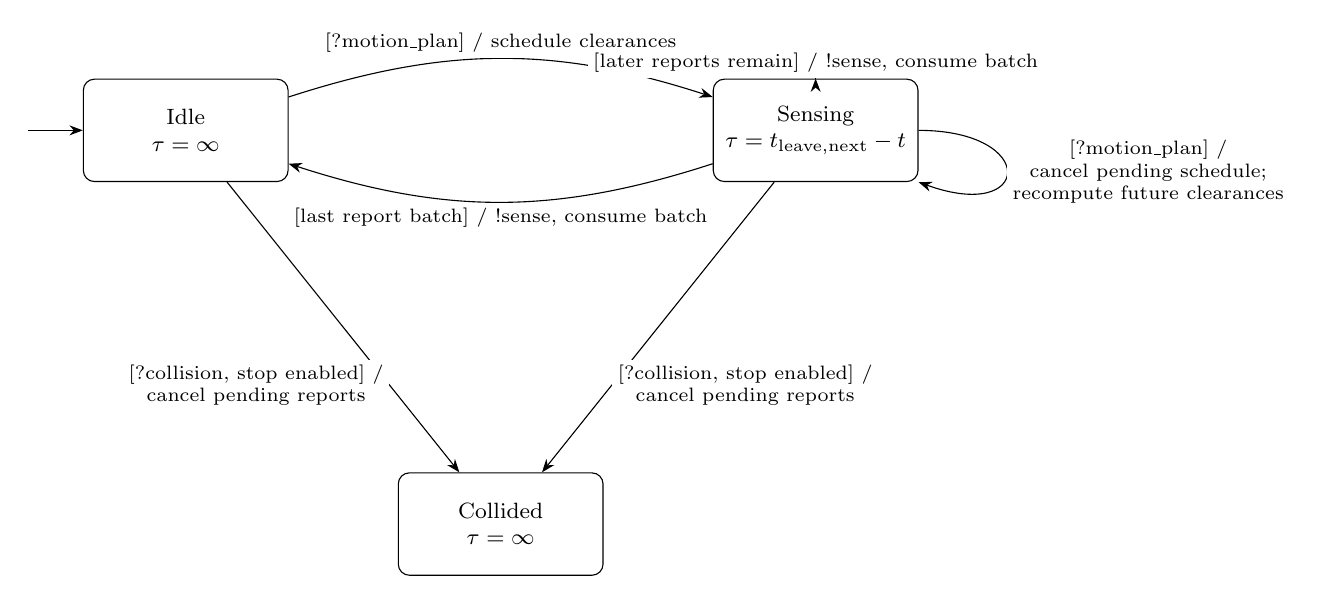
\begin{tikzpicture}[>=Stealth,every node/.style={font=\footnotesize},
 phase/.style={draw,rounded corners,align=center,minimum width=26mm,minimum height=13mm},
 lab/.style={align=center,fill=white,inner sep=2pt,font=\scriptsize}]
\node[phase] (i) at (0,0) {Idle\\$\tau=\infty$};
\node[phase] (s) at (8,0) {Sensing\\$\tau=t_{\rm leave,next}-t$};
\node[phase] (c) at (4,-5) {Collided\\$\tau=\infty$};
\draw[->] (-2,0)--(i);
\draw[->] (i) to[bend left=18] node[lab,above]{[?motion\_plan] / schedule clearances}(s);
\draw[->] (s) to[bend left=18] node[lab,below]{[last report batch] / !sense, consume batch}(i);
\draw[->] (s.north) to[out=60,in=120,looseness=10] node[lab,above]{[later reports remain] / !sense, consume batch}(s.north);
\draw[->] (s.east) to[out=0,in=-20,looseness=6] node[lab,right]{[?motion\_plan] /\\cancel pending schedule;\\recompute future clearances}(s.south east);
\draw[->] (i)--node[lab,left,pos=.7]{[?collision, stop enabled] /\\cancel pending reports}(c);
\draw[->] (s)--node[lab,right,pos=.7]{[?collision, stop enabled] /\\cancel pending reports}(c);
\end{tikzpicture}}
\caption{PSensor phase transitions in the implemented model. With no
pending clearance, Sensing has infinite time advance.}
\label{fig:psensor-phases}
\end{figure}
With collision stopping disabled, PSensor ignores collision inputs and
MRobot continues its motion while displaying its collision status. The
validation runs use collision stopping. The diagrams describe the current
implementation: PSensor enters Collided directly; it does not currently
emit a separate collision-report transition.

\clearpage
\subsection{Release-driven destination extension without lookahead}
This optional extension remains experimental and is disabled in the current
reported stop-only baseline. The controller initiates an extension only after actual Plant clearance
reports make the next portion of the prescribed path admissible. TrafficManager
retains FIFO selection and required precedence checks, reserves the new approved
portion in RoadMap, and buffers a command for RMFSController to emit.
It does not predict a collision-free timing gap and it does not wait for a
pre-braking request from MRobot: the \texttt{!motion\_status} port and its
request/response protocol have been removed.

\begin{figure}[htbp]
\centering
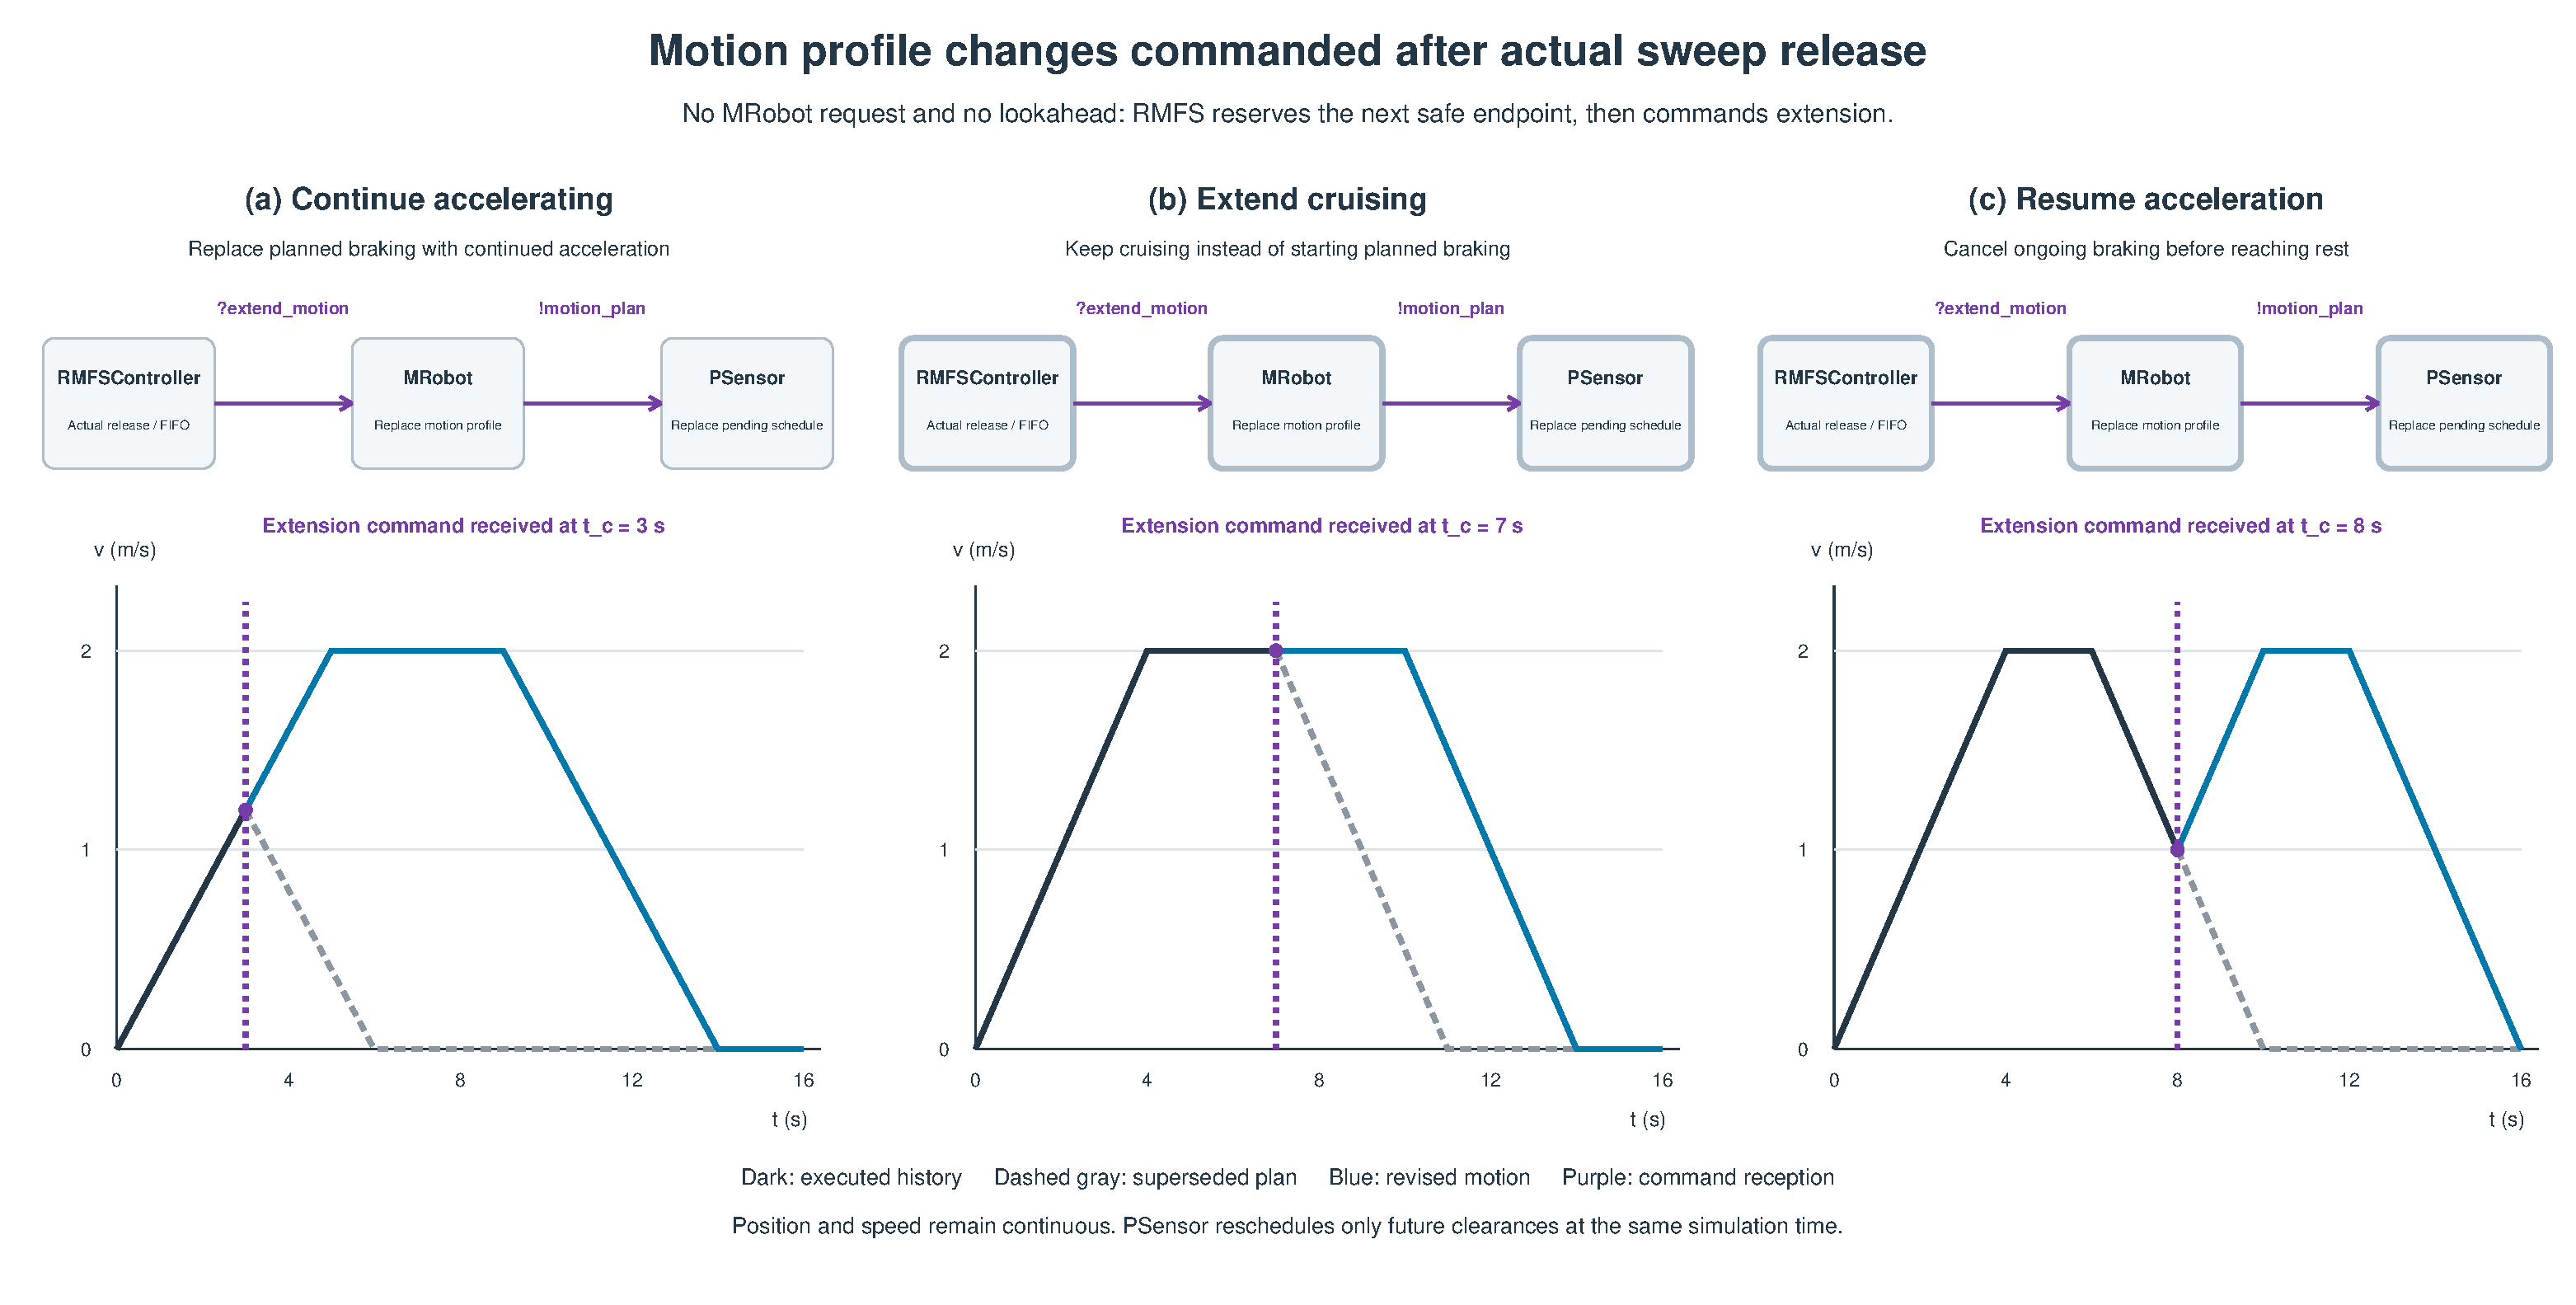
\includegraphics[width=\linewidth]{motion_profile_changes.pdf}
\caption{Controller-commanded motion changes after actual sweep release.
The purple marker is the reception time of an extension command, not a
scheduled profile-transition deadline. MRobot immediately preserves the
executed prefix and replaces its future profile; its zero-time
\texttt{!motion\_plan} output updates PSensor. Curves illustrate acceleration
continuation, cruise extension, and reacceleration during braking; they are
schematic profiles, not measured benchmark traces.}
\label{fig:release-driven-profile}
\end{figure}

Figure~\ref{fig:release-driven-profile} illustrates three physical responses
to the same command. During acceleration the robot can continue accelerating;
during cruise it can postpone braking; during deceleration it can accelerate
again without first reaching zero speed. Commands extend the current final
straight run in its existing direction. A turn still requires the existing
stop-and-rotate behavior. If the robot has already stopped, the controller
issues an ordinary new movement command. Without an extension, the original
stop remains in force.

Let $t_c$ be the reception time, $u=v(t_c)$ the current speed, $D$ the
remaining straight distance to the newly approved endpoint, $a,b>0$ the
acceleration and braking magnitudes, and $v_{\max}$ the speed limit.
For $D\ge u^2/(2b)$, the replacement tail uses
\begin{equation}
 w=\min\!\left(v_{\max},
 \sqrt{\frac{2D+u^2/a}{1/a+1/b}}\right),\qquad
 t_a=\frac{w-u}{a},\qquad
 t_v=\frac{D-(w^2-u^2)/(2a)-w^2/(2b)}{w}.
 \label{eq:extension-tail}
\end{equation}
Here $w$ is the new peak speed, $t_a$ the acceleration duration and $t_v$
the cruise duration (zero for a triangular tail). The final braking duration
is $w/b$. Position and speed are continuous at $t_c$; the permitted
acceleration can change at that event. In the implementation,
\texttt{ExtendedProfile} retains the original distance-time function for
the executed prefix and splices this tail at $t_c$.

\paragraph{Sensor schedule replacement.}
At the same simulation time, MRobot emits the revised motion plan, including
the profile, original run origin and time, direction, all intermediate path
points and footprint half-sizes. PSensor cancels its unreported reservations
and recomputes clearance times using the revised inverse distance function.
It retains only events strictly later than $t_c$; elapsed clearances are not
reported twice. A point already behind the centre but still under the footprint
remains eligible for its future clearance report. Endpoint occupancy is never
released merely because the centre arrives. These events update RoadMap and
reconsider FIFO waiters while the leading robot may still be moving.
The model snapshot includes the revised profile, pending zero-time output and
PSensor schedule, so restoration reproduces the same remaining execution.

\paragraph{Executable inspection.}
The three-robot example below uses the ordinary DEVS engine,
actual release reports, FIFO and sweep merging; it performs no lookahead.
Run it with
\begin{quote}\small\ttfamily
python -m examples.RMFS.Tests.03\_09\_RobotPath\_FIFO\_ReleaseExtension
\end{quote}
Space advances one event; A toggles automatic playback and R resets.
In the empty-robot case, R2 starts braking at $8.000$ s. R1's clearance on
arrival at $9.878$ s authorizes extension while R2 is still braking.
R2 then reaccelerates from its nonzero speed and PSensor replaces the pending
clearance schedule. The sampled stop-on-collision validation uses $0.1$ s
intervals and all three routes finish without detected contact at $25.101$ s.
This is a reproducible example, not a general continuous-time collision proof.

\end{document}





